

\documentclass[NETN,manuscript]{stjour-new}

\usepackage{comment}
\usepackage{booktabs}
\usepackage{pbox}
\usepackage{afterpage}
\usepackage{makecell}
\usepackage{fourier} 
\usepackage{array}
\usepackage{xr}
\usepackage{cleveref}
%\usepackage{adjustbox}
\usepackage{tikz-cd}
\usepackage{graphics}
%\usepackage{adjustbox}
\usepackage[english]{babel}
\usepackage[utf8]{inputenc}
\usepackage{algorithm}
\usepackage{tikz-cd}
\usepackage{graphicx}
\usepackage{subfig}
\usepackage[export]{adjustbox}
\newlength\Colsep
\setlength\Colsep{10pt}
\usetikzlibrary{arrows.meta,
                positioning
                }
%\externaldocument[supp-]{Supplement.tex}


\newcommand{\skcomment}[1]{({\color{blue}{SK's comment:}}\textbf{\color{blue}{#1}})}
\renewcommand\theadalign{bc}
\renewcommand\theadfont{\bfseries}
\renewcommand\theadgape{\Gape[4pt]}
\renewcommand\cellgape{\Gape[4pt]}

\makeatletter
\newcommand*{\addFileDependency}[1]{% argument=file name and extension
  \typeout{(#1)}% latexmk will find this if $recorder=0 (however, in that case, it will ignore #1 if it is a .aux or .pdf file etc and it exists! if it doesn't exist, it will appear in the list of dependents regardless)
  \@addtofilelist{#1}% if you want it to appear in \listfiles, not really necessary and latexmk doesn't use this
  \IfFileExists{#1}{}{\typeout{No file #1.}}% latexmk will find this message if #1 doesn't exist (yet)
}
\makeatother

\newcommand*{\myexternaldocument}[1]{%
    \externaldocument{#1}%
    \addFileDependency{#1.tex}%
    \addFileDependency{#1.aux}%
}
\myexternaldocument{Supplement}
\listfiles

\articletype{Research}

\def\taupav{\tau_{\mathrm{Pav}}}

\begin{document}

%\afterpage{%
%   \clearpage % flush any accumulated floats
%   \begin{figure}[ht!]  % or: \begin{table}[ht!]
%   ... % body of figure/table environment
%   \end{figure} % or: \end{table}
%} % end of scope of \afterpage directive

\title{Modelling the cell-type specific murine connectome}
%\subtitle{mouse connectome} %% Optional subtitle

\author[Koelle et al]% shortened version for running head, optional
{Samson Koelle \affil{1,2}, Jennifer Whitesell \affil{1}, Karla Hirokawa \affil{1},  Hongkui Zeng\affil{1}, Marina Meila\affil{2}, Julie Harris\affil{1}, Stefan Mihalas\affil{1}}

\affiliation{1}{Allen Institute for Brain Science, Seattle, WA, USA}

\affiliation{2}{Department of Statistics, University of Washington, Seattle, WA, USA}

\correspondingauthor{Stefan Mihalas}{stefanm@alleninstitute.org}

\keywords{[a series of capitalized words, separated with commas]}

\begin{abstract}

The Allen Brain Connectivity Atlas consists of thousands of labelling experiments targeting interrogating diverse structures and classes of projecting neurons.
This paper describes the conversion of these experiments into class-specific connectivity matrices representing the connection between source and target structures.
We introduce and validate a novel statistical model for creation of connectivity matrices that combines spatial and categorical smoothing to share information between similar neuron classes.
We then illustrate overall and cell-type specific connectivity patterns in the resultant connectivities.

\end{abstract}

\begin{authorsummary}
\end{authorsummary}

\section{Introduction}
 
The mammalian nervous system enables an extraordinary range of natural behaviors, and has inspired much of modern artificial intelligence.
Neural connections including those from one region to another form the architecture underlying this capability.
These connectivities vary by neuron type, as well as source (cell body) location and target (axonal projection) structures.
Thus, characterization of the relationship between neuron type and source and target structure is important for understanding the overall nervous system.

Viral tracing experiments - in which a viral vector expressing GFP is transduced into neural cells through stereotaxic injection - are a useful tool for mapping these connections on the mesoscale \citep{Chamberlin1998-hi,Harris2012-fw, Daigle2018-gd}.
The long range connections between different areas are generally formed by axons which travel from one region to another, and the GFP protein moves into the axon of the projecting neurons.
Two-photon tomography imaging can be used to determine the location and strength of the fluorescent signals in two-dimensional slices.
These locations can then be mapped back into three-dimensional space, and the signal may then be integrated over area into cubic voxels to give a finely-quantized three-dimensional fluorescence.

Several statistical models for the conversion of such experiment-specific signals into generalized estimates of connectivity strength have been proposed \citep{Oh2014-kh, Harris2016-fn, Gamanut2018-sd, Knox2019-ot}.
Of these, \citet{Oh2014-kh} and \citet{Knox2019-ot} provide a model for \textbf{regionalized connectivities}, which are voxel connectivities integrated by region.
The value of these models is that they provide some improvement over simply averaging the projection signals of injections in a given region.
However, these previous works only model connectivities observed in wild-type mice which are suboptimally suited to assessment of cell-type specific connectivity compared with fluorescence from Cre-recombinase induced eGFP expression in cell-types specified by the combination of transgenic mouse strain and transgene promoter \citep{Harris2019-mr}.
We generally refer to sets of so-targeted eGFP-expressing cells in tracing experiments as a \textbf{cell class} since they may contain multiple types.
For example, use of both wild-type and transgenic mice would give rise to cell-class specific experiments, albeit with different yet perhaps overlapping classes of cells.

Thus, this paper introduces a class-specific statistical model for anterograde tracing experiments that synthesizes the diverse set of \textbf{Cre-lines} described in \citet{Harris2019-mr}, and expands this model to the entire mouse brain.
Our model is a to-our-knowledge novel statistical estimator that takes into account both the spatial position of the labelled source, as well as the categorical cell class.
Like the previously state-of-the-art model in \citet{Knox2019-ot}, this model predicts regionalized connectivity as an average over positions within the structure, with nearby experiments given more weight.
However, our model weighs class-specific behavior in a particular structure against spatial position, so a nearby experiment specific to a similar cell-class is relatively up-weighted, while a nearby experiment specific to a dissimilar class is down-weighted.
This model outperforms the model of  \citet{Knox2019-ot} based on its ability to predict held-out experiments in leave-one-out cross-validation.
We use the trained model to estimate overall connectivity matrices for each assayed cell class.

The resulting cell-class specific connectivity is a directed weighted multigraph which can be represented as a tensor with missing values.
We do not give an exhaustive analysis of this data, but do establish a lower-limit of detection, verify several cell-type specific connectivity patterns found elsewhere in the literature, and show that these cell-type specific signals are behaving in expected ways.
We also decompose the wild-type connectivity matrix into factors representing latent connectivity patterns, which we call archetypes.
These components allow approximation of the regionalized connectivity using linear combinations of a small set of components.

Section \ref{sec:methods} gives information on the data and statistical methodology, and Section \ref{sec:results} presents our results.
These include connectivities, assessments of model fit, and subsequent biological and statistical analyses.
Additional information on our dataset, methods, and results are given in Supplemental Sections \ref{supp_sec:info}, \ref{supp_sec:methods}, and \ref{supp_sec:exp}, respectively.
\section{Methods}
\label{sec:methods}

We estimate and analyze cell class-specific connectivity functions using models trained on murine brain viral tracing experiments.
This section describes the data used to generate the model, the model itself, the evaluation of the model against its alternatives, and the use of the model in creation of the connectivity estimate matrices.
It also includes background on the non-negative matrix factorization method used for decomposing the wild type connectivity matrix into latent factors.
Additional information about our data and methods are given in Supplemental Sections \ref{supp_sec:data} and \ref{supp_sec:methods}, respectively.

\newpage
\begin{figure}[H]
\subfloat[]{
\label{fig:mouse}
    
\includegraphics[width=0.3\textwidth]{figs/figure1a.png}}
\subfloat[]{
\label{fig:injproj}
    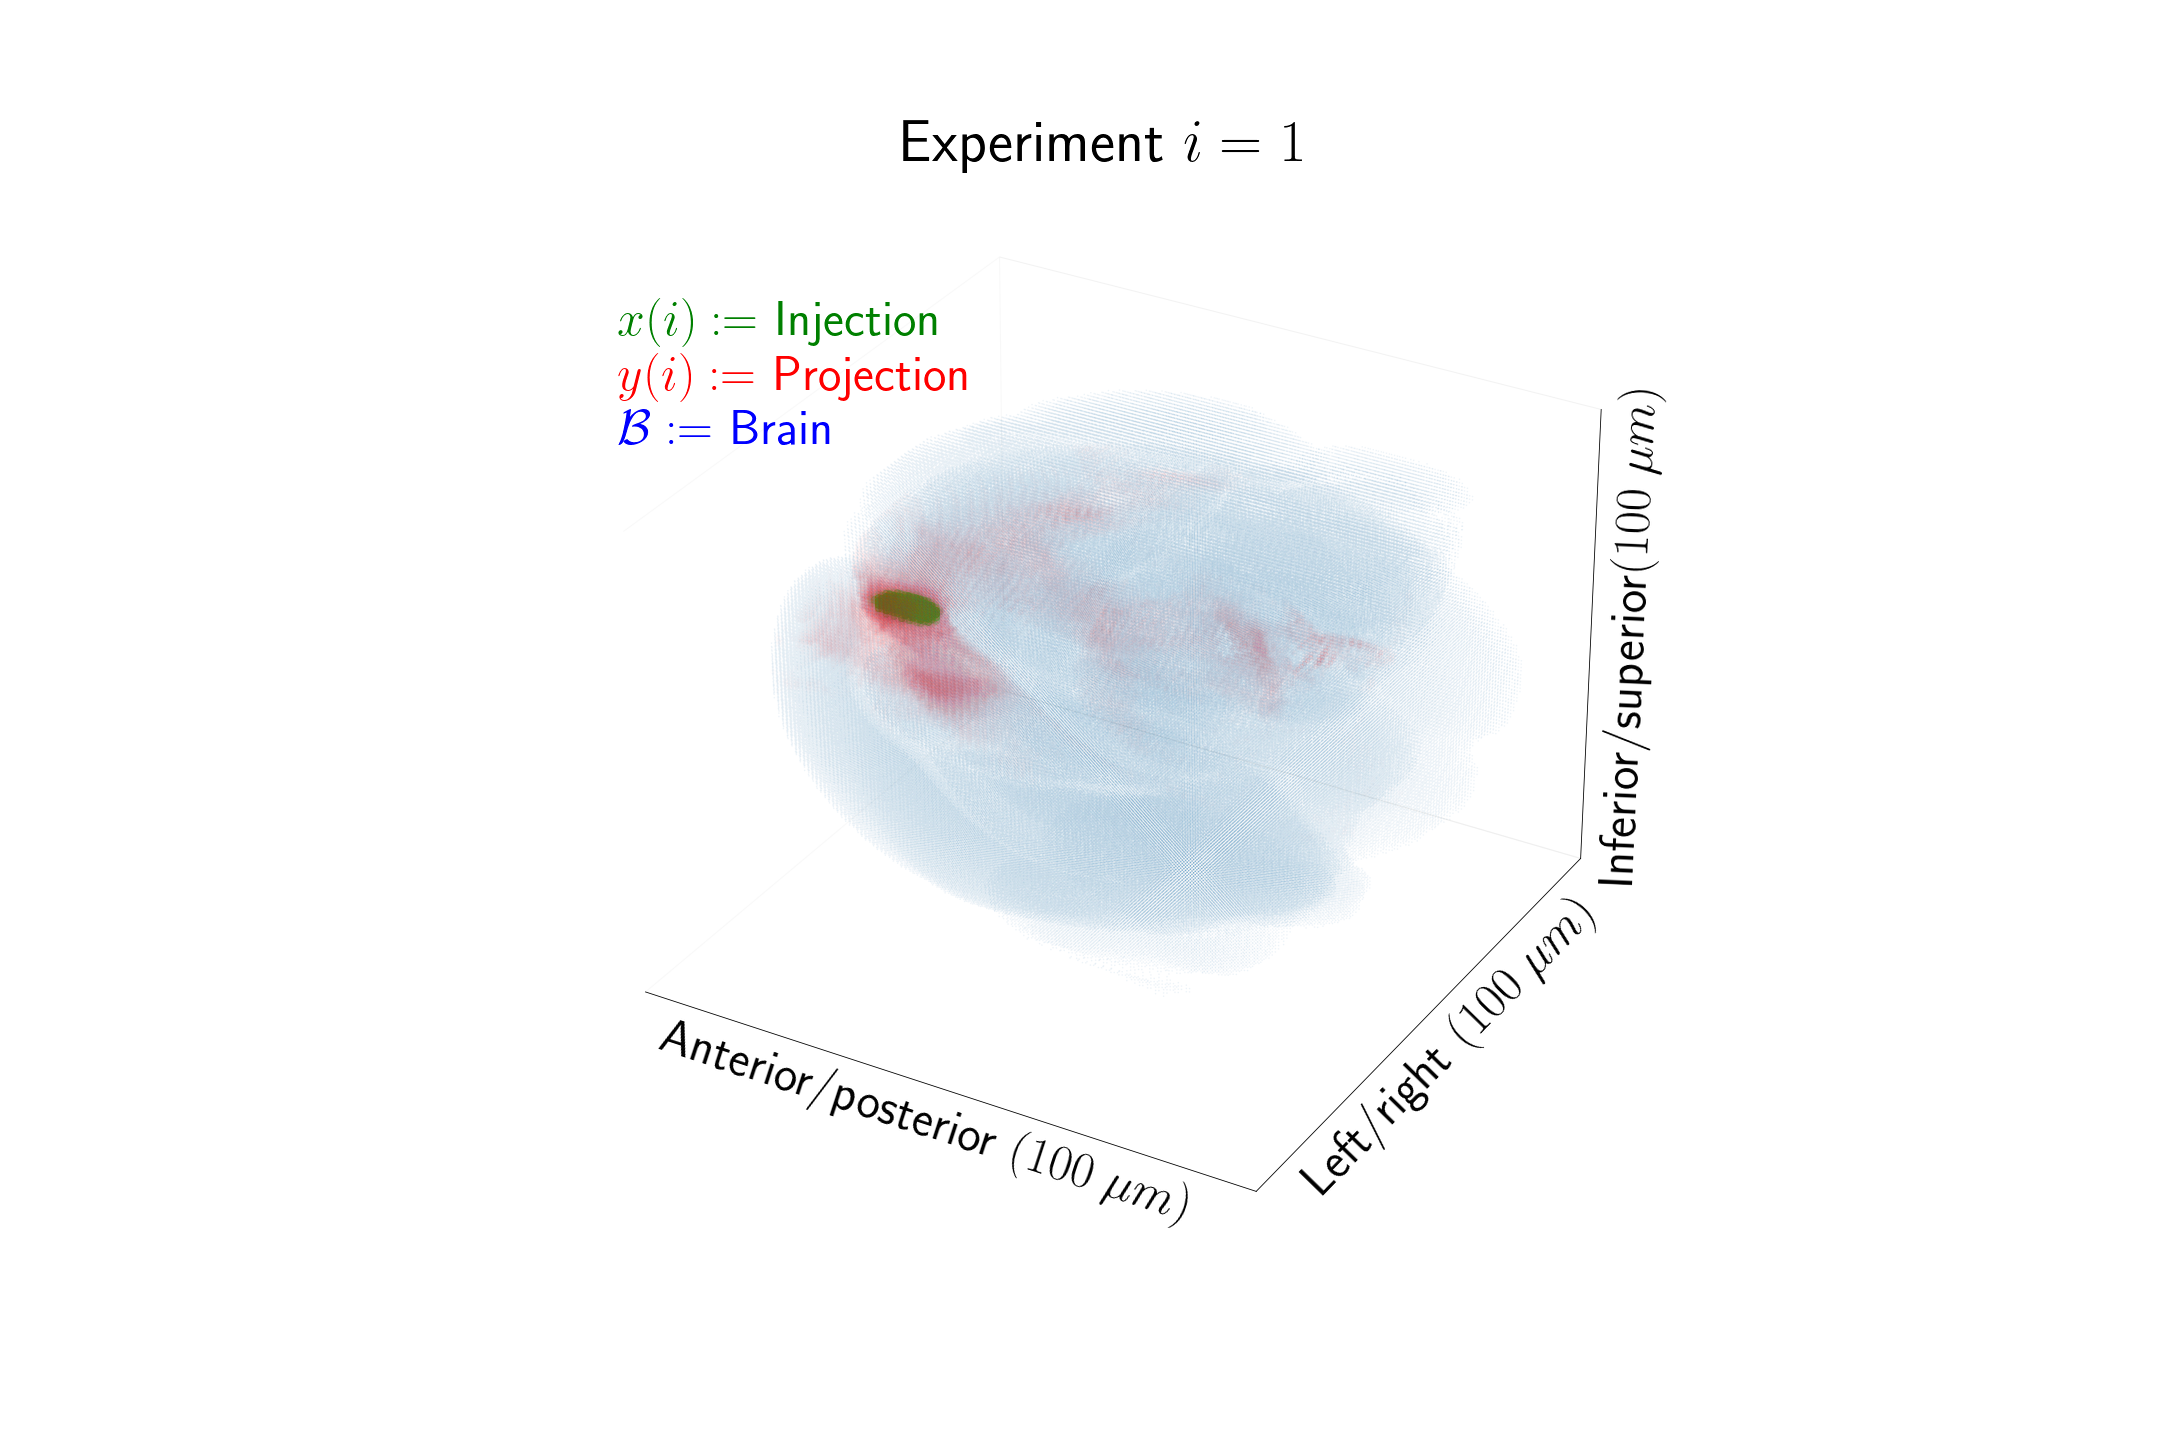
\includegraphics[width=0.4\textwidth]{figs/inj_proj_figure_v2.png}}
\subfloat[]{
\label{fig:segment}
    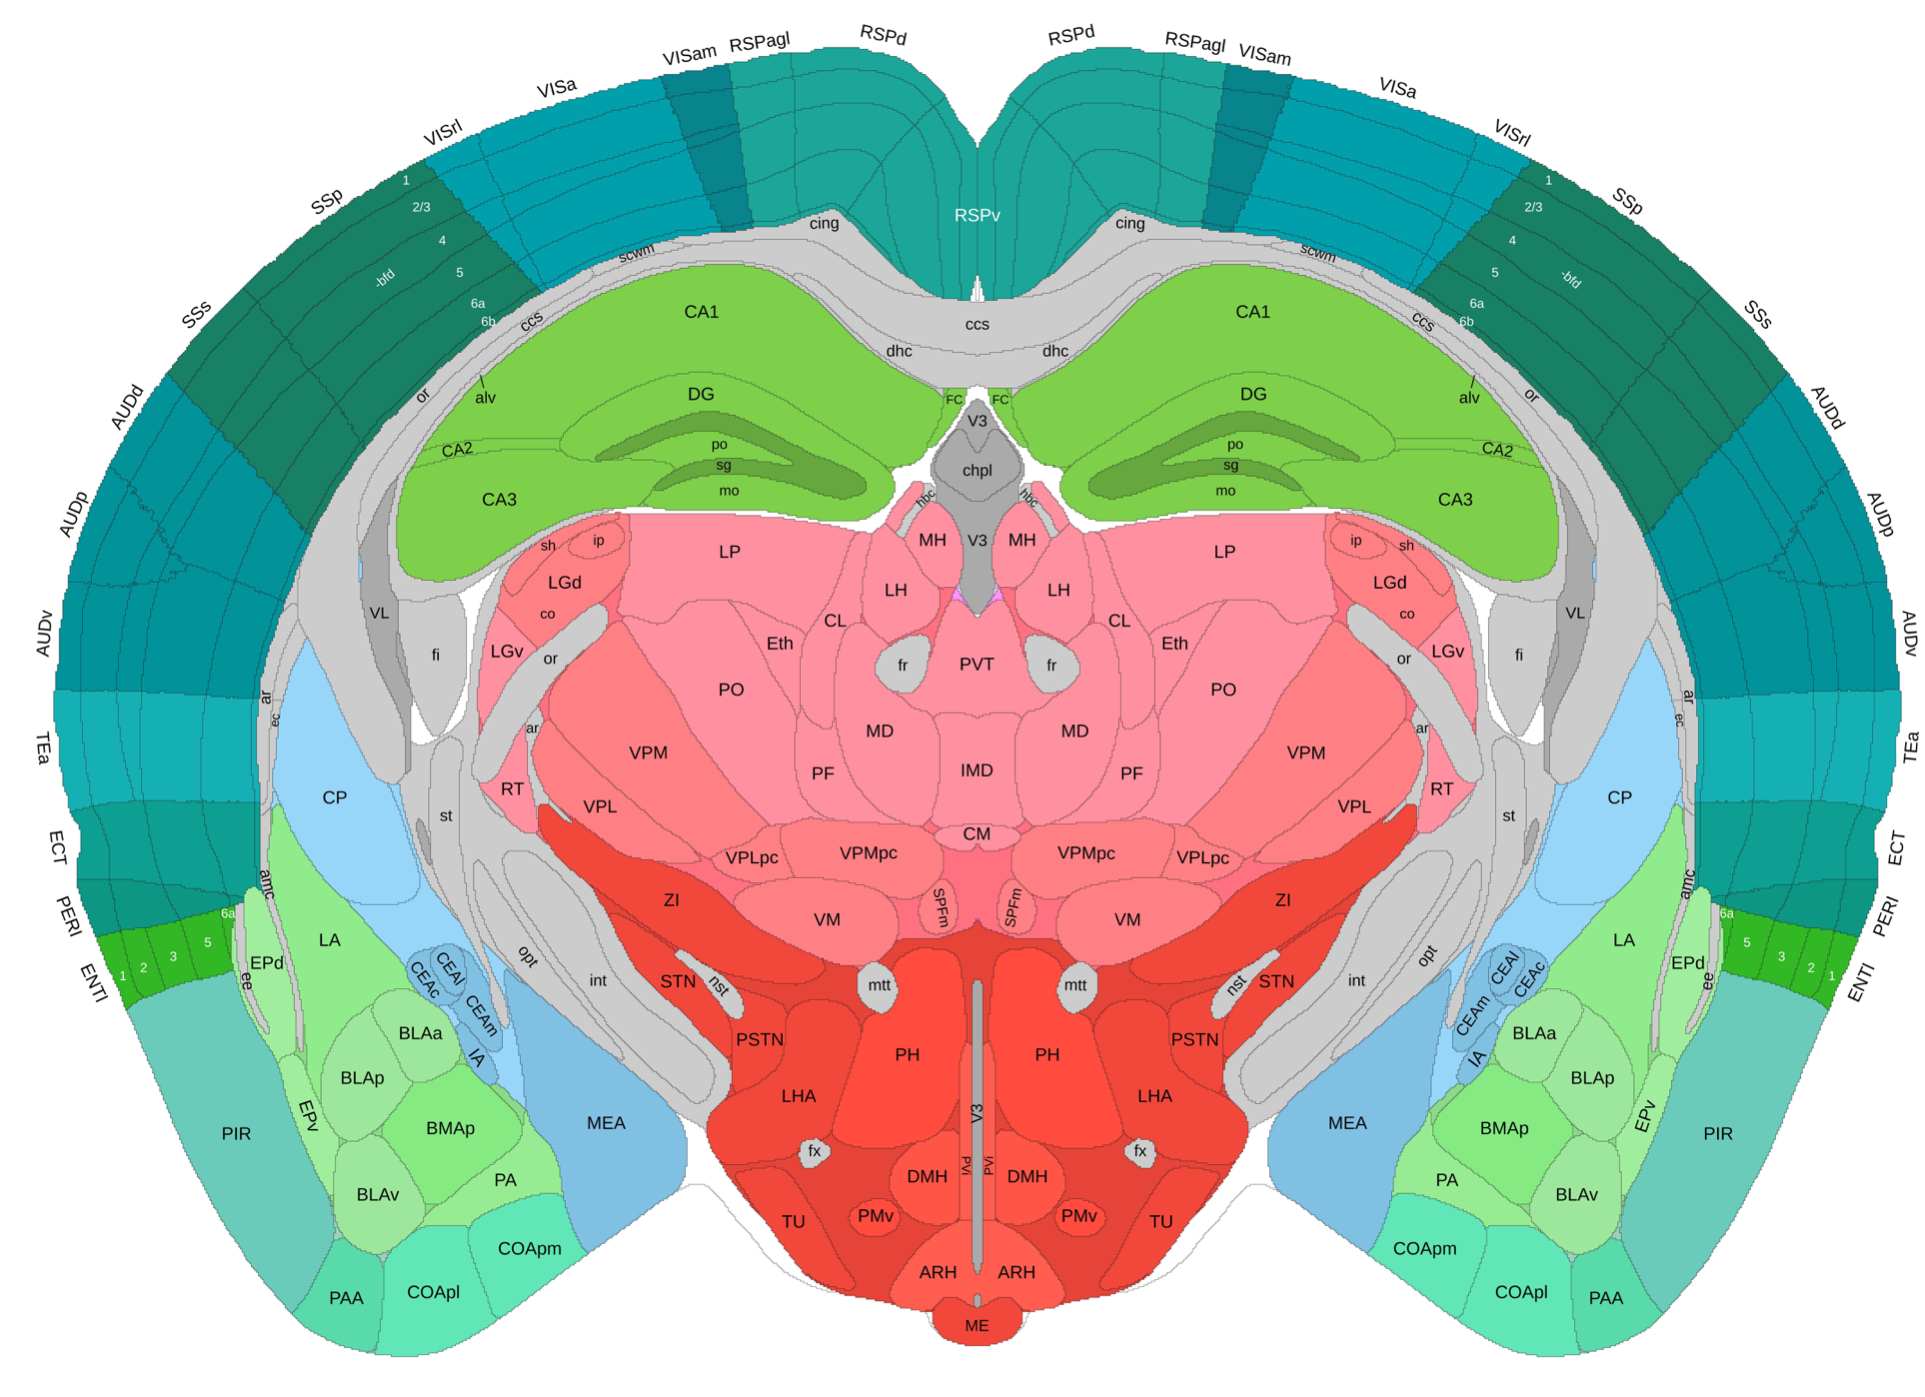
\includegraphics[width=0.3\textwidth]{figs/fig1c.png}}
    \newline
 \subfloat[]{
 \label{fig:ontology}
    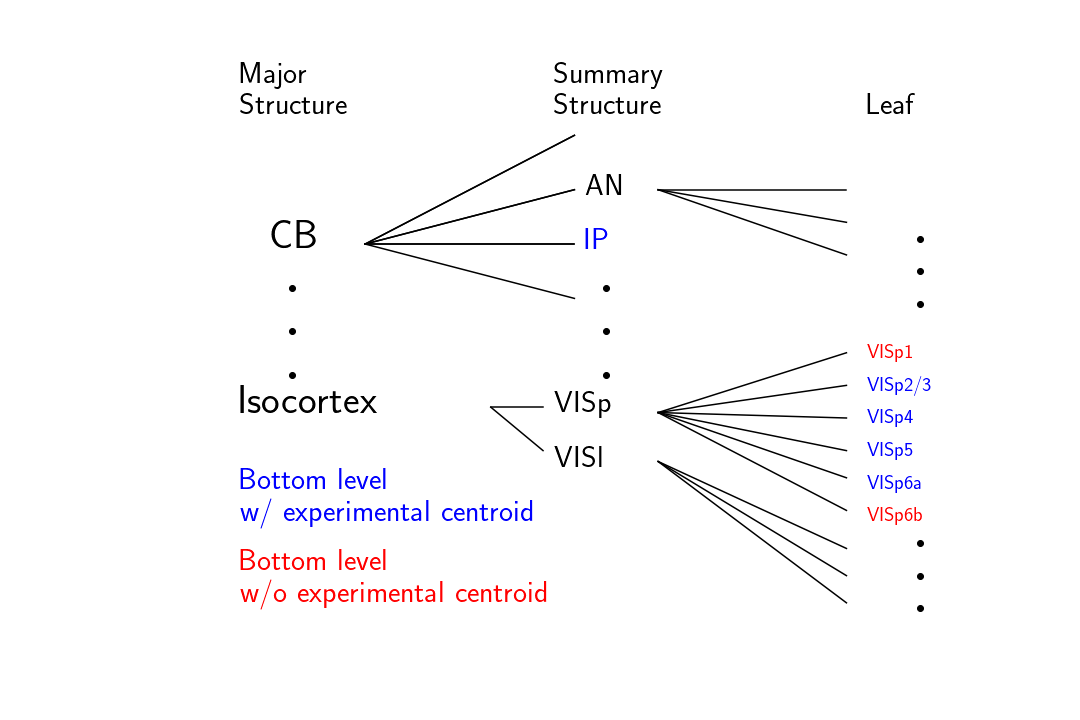
\includegraphics[width=0.35\textwidth]{figs/ontologyfigure.png}}
\subfloat[]{
 \label{fig:top}
    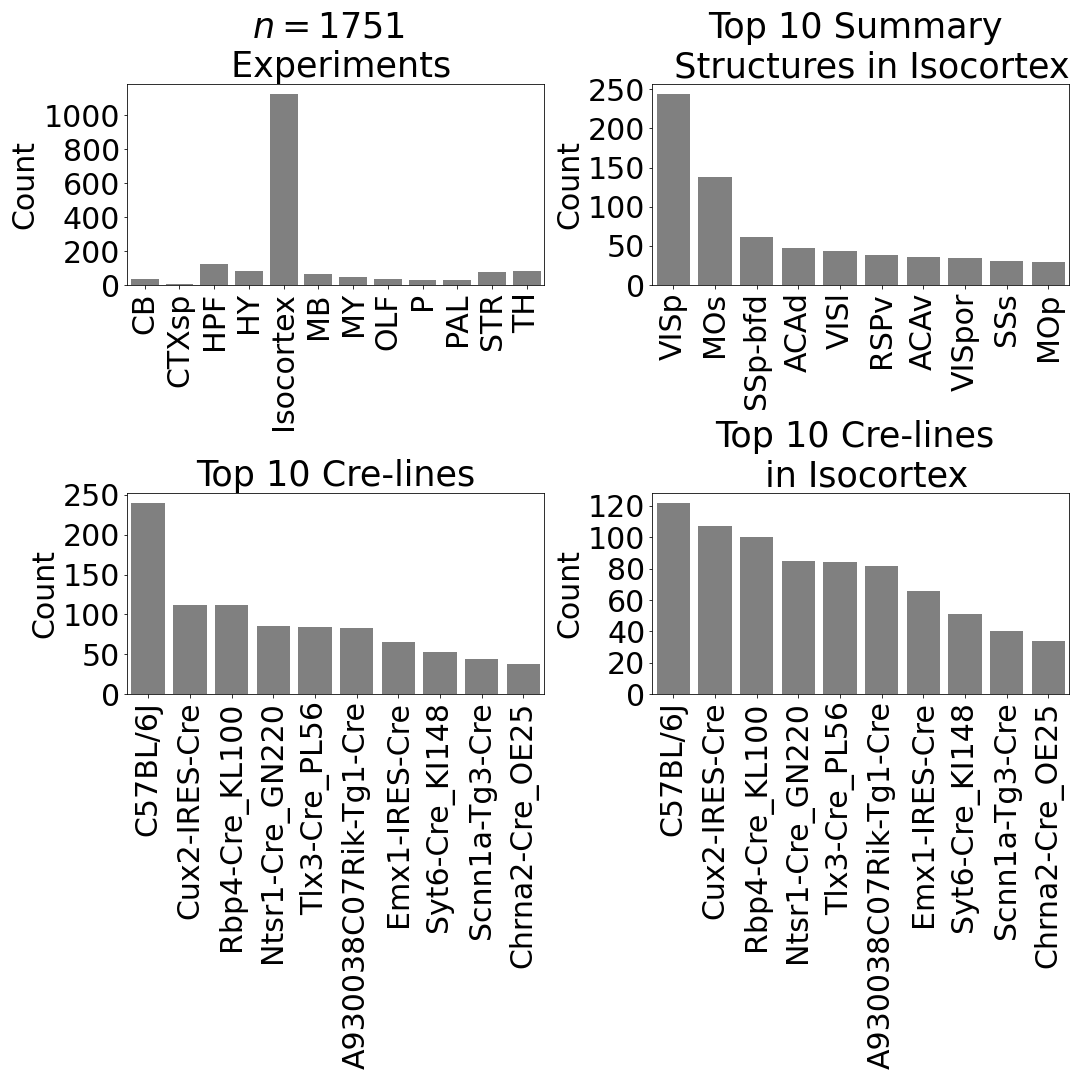
\includegraphics[width=0.35\textwidth]{figs/datasummary.png}}
\subfloat[]{
 \label{fig:combos}
    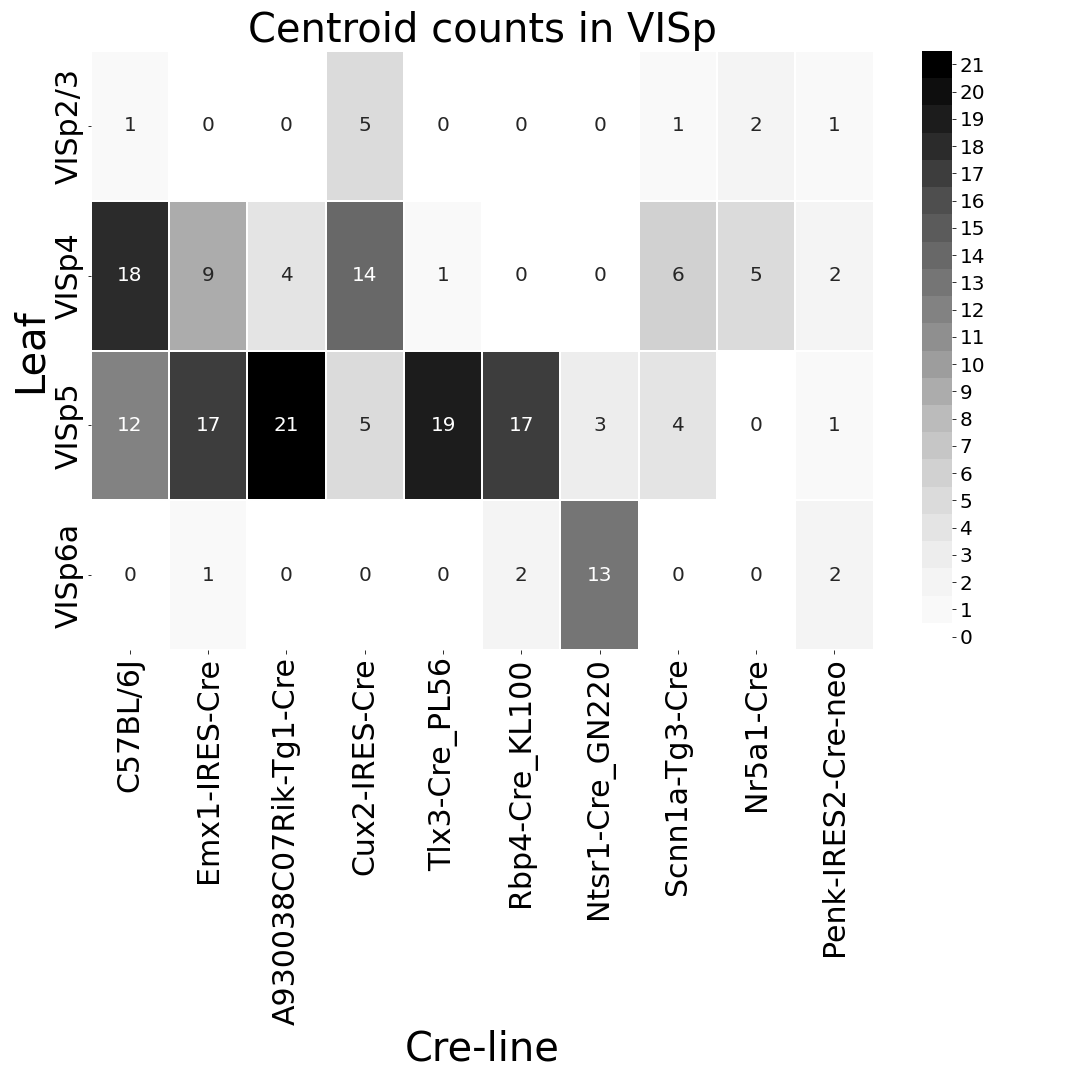
\includegraphics[width=0.35\textwidth]{figs/visp_counts.png}}   
    \caption{Experimental setting.  \ref{fig:mouse}  For each experiment, a Cre-dependent GFP-expressing transgene casette is transduced by stereotaxic injection into a Cre-driver mouse, followed by serial two-photon tomography imaging.
    \ref{fig:injproj} An example of the segmentation of projection (targets) and injection (source) for a single experiment. Within each brain (blue), injection (green) and projection (red) areas are determined via histological analysis and alignment to the Allen Common Coordinate Framework (CCF).
    \ref{fig:segment} Brain region parcellations within a coronal plane of CCFv3. \ref{fig:ontology} Explanation of nested structural ontology highlighting various levels of CCFv3 structure ontology.
    Lowest-level (leaf) structures are colored in blue, and structures without an injection centroid are colored in red.
    \ref{fig:top}  Abundances of tracer experiments by Cre-line and region of injection. \ref{fig:combos}  Co-occurrence of layer-specific centroids and Cre-lines within VISp.}
    \label{fig:data}
\end{figure}

\newpage

\subsection{Data}

Our dataset $\mathcal D$ consists of $n=1751$ publicly available murine brain viral tracing experiments from the Allen Mouse Brain Connectivity Atlas.
Figure \ref{fig:mouse} summarizes the experimental process used to generate this data.
In each experiment, a mouse is injected with an adeno-associated virus (AAV) encoding green fluorescent protein (GFP) into a single location in the brain.
Location of fluorescence is mediated by the location of the injection, the characteristics of the transgene, and the genotype of the mouse.
In particular, Cre-driver mice are engineered to express Cre under the control of a specific and single gene promoter.
This localizes expression of Cre to regions with certain transcriptomic cell-types signatures.
In such Cre-driver mice, we used a double-inverted floxed AAV to produce fluorescence that depends on Cre expression in infected cells.
To account for the complex cell-type targeting induced by a particular combination of Cre-driver genotype and GFP promoter, we refer to the combinations of cell-types targeted by a particular combination of AAV and Cre-driver mice as cell-classes.
For example, we include experiments from Cre-driver lines that selectively label cell classes located in distinct cortical layers or other nuclei across the whole brain.
By our definition, wild type mice transduced with constitutitively active GFP promoters induce fluorescence of a particularly broad cell class.

For each experiment, the fluorescent signal imaged after injection is aligned into the Allen Common Coordinate Framework (CCF) v3, a three-dimensional average template brain that is fully annotated with regional parcellations \cite{Wang2020-po}.
The whole brain imaging and registration procedures described in detail in \citet{Oh2014-kh, Kuan2015-zz} produce quantitative metrics of fluorescence discretized at the $100 \; \mu$m \textbf{voxel} level. 
Given an experiment, this image was histologically segmented by an analyst into \textit{injection} and \textit{projection} areas corresponding to areas containing somas, dendrites and axons or exclusively axons of the transfected neurons.
An example of a single experiment rendered in 3D is given in Figure \ref{fig:injproj}.
Given an experiment $i$, we represent injections and projections as functions $x(i),y(i) : \mathcal B \to \mathbb R_{\geq 0}$, where $\mathcal B \subset [1:132] \times [1:80] \times [1:104]$ corresponds to the subset of the $(1.32 \times 0.8 \times 1.04)$ cm rectangular space occupied by the standard voxelized mouse brain.
We also calculate injection centroids $c(i) \in \mathbb R^3$ and regionalized projections $y_{\mathcal T} (i) \in \mathbb R^{T} $ given by the sum of $y(i)$ in each region.
A description of these steps is in Supplemental Section \ref{supp_sec:dp}.

Our goal is the estimation of \textbf{regionalized connectivity} from one region to another.
A visual depiction of this region parcellation for a two-dimensional slice of the brain is given in Figure \ref{fig:segment}.
All structures annotated in the CCF belong to a hierarchically ordered ontology, with different areas of the brain are parcellated to differing finer depths within a hierarchical tree.
We denote the main levels of interest as major structures, summary structures, and layers.
Not every summary structure has a layer decomposition within this ontology, so we typically consider the finest possible regionalization - for example, layer within the cortex, and summary structure within the thalymus, and denote these structures as leafs.
As indicated in Figure \ref{fig:ontology}, the dataset used to generate the connectivity model reported in this paper contains certain combinations of region and cell class frequently, and others not at all.
A summary of the most frequently assayed cell classes and structures is given in Figures \ref{fig:top} and \ref{fig:combos}.
Since users of the connectivity matrices may be interested in particular combinations, or interested in the amount of data used to generate a particular connectivity estimate, we present this information about all experiments in Supplemental Section \ref*{supp_sec:data}.

\newpage

\subsection{Modeling Regionalized Connectivity}
\label{sec:modelling}

We define voxelized cell-class specific connectivity $f:  \mathcal V \times \mathcal B \times \mathbb \mathcal \to \mathbb R_{\geq 0}$ as giving the voxelized connectivity strength of a particular cell class from a source voxel to a target voxel.
In contrast to \citet{Knox2019-ot}, which only uses wild type C57BL/6J mice, our dataset has experiments targeting $|\mathcal V| = 114$ different combinations of Cre-driver mice and Cre-regulated AAV transgenes jointly denoted as $\mathcal V := \{v\}$.
As in \citet{Knox2019-ot}, we ultimately estimate an integrated regionalized connectivity defined with respect to a set of $S = 564$ source leafs $\mathcal S := \{ s\} $ and $T = 1123$ target leafs $\mathcal T := \{ t \}$, of which $1123 - 564  = 559$ are contralateral.
That is, we define
\begin{align*}
&\text{\textit {regionalized connectivity strength} } \mathcal C : \mathcal V \times \mathcal S \times \mathcal T \to \mathbb R_{\geq 0}  \text{ with } \mathcal C(v,s,t) = \sum_{l_{j} \in s} \sum_{l_{j'} \in  t} f(v,l_{j},l_{j'}), \\
&\text{\textit {normalized regionalized connectivity strength} } \mathcal C^N : \mathcal V \times \mathcal S \times \mathcal T \to \mathbb R_{\geq 0}  \text{ with } \mathcal C^N(v,s,t) = \frac{1}{|s|} \mathcal C(v,l_{j},l_{j'}), \\
&\text{\textit {normalized regionalized projection density} } \mathcal C^D : \mathcal V \times \mathcal S \times \mathcal T \to \mathbb R_{\geq 0} \text{ with } \mathcal C^D(v,s,t) = \frac{1}{| s | | t|}\mathcal C(v,l_{j},l_{j'})
\end{align*}
where $l_j$ and $l_{j'}$ are the locations of source and target voxels, and $|s|$ and $|v|$ are defined to be the number of voxels in the source and target structure, respectively.
Since the normalized strength and densities are computable from the strength via a fixed normalization, our main statistical goal is to estimate $\mathcal C (v,s,t) $ for all $v, s$ and $t$.% and density are
In other words, we want to estimate matrices $\mathcal C_v \in \mathbb R_{\geq 0}^{S \times T}$.
We call this estimator $\widehat { \mathcal C } $.

Construction of such an estimator raises the questions of what data to use for estimating which connectivity, how to featurize the dataset, what statistical estimator to use, and how to reconstruct the connectivity using the chosen estimator.
We represent these considerations as 
\begin{align}
\label{eq:estimator}
\widehat { \mathcal C }(v,s,t) = f^* (\widehat f (f_*( \mathcal D(v,s))).
\end{align}
This makes explicit the data featurization $f_{*}$, statistical estimator $\widehat f$, and any potential subsequent transformation $f^*$ such as summing over the source and target regions.
Denoting $ \mathcal D$ as a function of $v$ and $s$ reflects that we consider using different data to estimate connectivities for different cell-classes and source regions.
Table \ref{tab:estimators} reviews estimators used for this data-type used in previous work, as well as our two main extensions: the Cre-NW and \textbf{Expected Loss} (EL) models.
The main differences in our data featurization from \citep{Knox2019-ot} are that we regionalize our data at the leaf level where available so that it layer-specific behavior is visible, and normalize our data by projection signal in order to account for differences between cell class.
Additional model selection results are given in Supplemental Section \ref{supp_sec:model-evaluation} for alternative normalization strategies, and more detail on estimation is given in Supplemental Section \ref{supp_sec:estimators}.

\begin{table}[H]
    \centering
    \begin{tabular}{c|c|c|c|c|}
        Name & $f^*$ & $\widehat f$&  $ f_*$ & $\mathcal D(v,s)$ \\
        \hline
        NNLS \citep{Oh2014-kh} & $\widehat f (1_s)$ & \nnls(X,Y) & $X= x_{\mathcal S},Y = y_{\mathcal T}$ & $ I_m / I_m$ \\
        NW \citep{Knox2019-ot} &$ \sum_{l_s \in s} \widehat f (l_s)$ & \nw(X,Y)  & $X = l_s, Y = y_{\mathcal T}$ & $I_m /I_m$ \\
        Cre-NW& $\sum_{l_s \in s} \widehat f(l_s)$ & \nw(X,Y) & $X= l_s, Y = y_{\mathcal T}$  &$ (I_l \cap I_v) / I_m$ \\
        Expected Loss (EL) & $\sum_{l_s \in s} \widehat f (s)$ & $\el(X,Y,v)$ & $X= l_s, Y = y_{\mathcal T}, v$  &$I_l / I_m$
    \end{tabular}
    \caption{Estimation of $\mathcal C$ using connectivity data.
    The regionalization, estimation, and featurization steps are denoted by $f^*, \widehat f,$ and  $f_*$, respectively.
    The training data used to fit the model is given by index set $I$.
    We denote experiments with centroids in particular major brain divisions and leafs as $I_m$ and $I_l$, respectively.
    Data $I_l / I_m$ means that, given a location $l_s \in s \in m$, the model $\widehat f$ is trained on all of $I_m$, but only uses $I_l$ for prediction.
    The non-negative least squares estimator (NNLS) fits a linear model that predicts regionalized projection signal $y_{\mathcal T}$ as a function of regionalized injection signal $x_{\mathcal S}$.
    Thus, the regionalization step for a region $s$ is given by applying the learned matrix $\widehat f$ to the $s$-th indicator vector.
    In contrast, the Nadaraya-Watson model (NW) is a local smoothing model that generates a prediction for each voxel within the source structure that are then averaged to create estimate the structure-specific connectivity.
    }
    \label{tab:estimators}
\end{table}

Our contributions - the Cre-NW and Expected Loss (EL) models - have several differences from the previous methods.
In contrast to the non-negative least squares \citep{Oh2014-kh} and Nadaraya-Watson  \citep{Knox2019-ot} estimators that account only for source region $s$, our new estimators account cell class $v$, 
The Cre-NW estimator only uses experiments from a particular class to predict connectivity for that class, while the EL estimator shares information between classes within a structure.
Both of these estimator take into account both the cell-class and the centroid position of the experimental injection.
Like the NW and Cre-NW estimator, the EL estimator generates predictions for each voxel in a structure, and then sums them together to get the overall connectivity.
However, in contrast to the NW approaches, the EL estimate of the projection vector for a cell-class at a location weights the average projection of that cell-class in the region containing the location against the relative locations of all experimental centroids in the region regardless of class.
That is, cell-class and source region combinations with similar average projection vectors will be upweighted when estimating $\widehat f$.
Thus, all experiments that are nearby in three-dimensional space can help generate the prediction, even when there are few nearby experiments for the cell-class in question.
A detailed mathematical description of our new estimator is given in Supplemental Section \ref{supp_sec:el}.

\newpage

\subsection{Model evaluation}

We select optimum functions from within and between our estimator classes using \textbf{leave-one-out cross validation}, in which the accuracy of the model is assessed by its ability to predict projection vectors experiments excluded from the training data on the basis of their cell class and experimental centroid.
Equation \ref{eq:estimator} includes a deterministic step $f^*$ included without input by the data.
The performance of $\widehat {\mathcal C} (v,s,t)$ is thus determined by performance of $\widehat f (f_*(\mathcal D(v,s)))$.
Thus, we evaluate prediction of $f_{\mathcal T}: \mathbb R^3 \to \mathbb R_{\geq 0}^T$ - the regionalized connection strength at a given location.

Another question is what combinations of $v, s, $ and $t$ to generate a prediction for.
Our EL and Cre-NW models are leaf specific.
They only generate predictions for cell-classes in leafs where at least one experiment with a Cre-line targeting that class has a centroid.
To accurately compare our new estimators with less-restrictive models such as used in \citet{Knox2019-ot}, we restrict our evaluation set to Cre driver/leaf combinations that are present at least twice. 
The sizes of these evaluation sets are given in Supplemental Section \ref{supp_sec:model-evaluation}.

We use weighted $l2$-loss to evaluate these predictions.
\begin{align*}
\text{l2-loss } \ell (y_{\mathcal T}(i)),\widehat {y_{\mathcal T}(i))}) &:=   \| y_{\mathcal T} (i)) - \widehat {y_{\mathcal T}(i))} \|_2^2. \\
\text{weighted l2-loss } \mathcal L ( \widehat {f(f_*)}) &:= \frac{1}{|\{\mathcal S,\mathcal V\}|} \sum_{s,v \in \{\mathcal S,\mathcal V\}} \frac{1}{ |I_{s} \cap I_v |} \sum_{i \in (I_{s} \cap I_v ) } \ell (y_{\mathcal T}(i)), \hat f_{\mathcal T} (f_*(\mathcal D(v,s) \setminus i)) .
\end{align*}
$I_s$ refers to the set of experiments with centroid in structure $s$, and $I_v$ refers to the set of experiments with Cre-line $v$, so $|I_s \cap I_v|$ is the number of experiments of Cre-line $v$ with injection centroid in structure $s$.
This is a somewhat different loss from \citet{Knox2019-ot} because of the increased weighting of rarer combinations of $s$ and $v$ implicit in the $\frac{1}{ |I_{s} \cap I_v |}$ term in the loss.
The establishment of a lower limit of detection and the extra cross-validation step used in the EL model to establish the relative importance of regionally averaged cell-class projection and injection centroid position are covered in Supplemental Section \ref{supp_sec:methods_lower}.

\newpage

\subsection{Connectivity analyses}

We examine latent structure underlying our estimated connectome using heirarchical clustering and non-negative matrix factorization.
First, we use aggloromative heirarchical clustering with Ward's criterion to compare outputs from connectivities from different Cre-lines.
Details of this approach are given in \citet{Hastie_2009, Lalloue2013-is}.
Second, we use non-negative matrix factorization (NMF) to factor the wild-type connectivity matrix into a small set of underlying components.
Inspired by \citet{Mohammadi2018-te}, we refer to these latent coordinates as \textbf{connectivity archetypes} since they represent underlying patterns from which we can reconstruct a broad range of observed connectivities, although we note that the genomic archetypal analysis in that paper is slightly methodologically distinct.

Our application of NMF to decompose the estimated long-range connectivity into latent coordinates that linearly combine to reproduce the observed connectivity is some independent interest, since we censor short range connections due to their clear biological derivation from diffusion and their high mathematical rank.
NMF refers to a collection of \textbf{dictionary-learning} algorithms for decomposing a non-negatively-valued matrix such as $\mathcal C $ into positively-valued matrices called, by convention, weights $W \in \mathbb R^{S \times q}_{\geq 0}$ and hidden units $H \in \mathbb R^{q  \times T}_{\geq 0}$.
NMF assumes a simple linear statistical model: that the observed matrix is composed of linear combinations of latent coordinates \citep{Devarajan2008-hd}.
Unlike PCA, NMF specifically accounts for the fact that data are all in the positive orthant, and it is more stable and interpretable in assays of complex biological systems than heirarchical clustering \citep{Brunet2004-gi}
The matrix $H$ is typically used to identify latent structures with interpretable biological meaning, and the choice of matrix factorization method reflects particular scientific subquestions and probabilistic interpretations. 

Our NMF algorithm solves the following optimization problem
\begin{eqnarray*}
\label{eq:nmf}
\nmf(\mathcal C, \lambda, q) := \arg \min_{W\in \mathbb R^{S \times q}_{\geq 0}, H \in \mathbb R^{q  \times T}_{\geq 0}} \frac{1}{2}\| 1_{d(s,t) > 1500 \mu m} \odot \mathcal C - WH\|_2^2  + \lambda  (\|H \|_1 + \|W \|_1) .
\end{eqnarray*}
For this decomposition we ignore connections between source and target regions less than  $1500 \mu m$ apart.
This is because short-range projections resulting from diffusion dominate the matrices $\hat {\mathcal C}$, and represent a less-interesting type of biological structure.
We set $\lambda = 0.002$ to encourage sparser and therefore more interpretable components.
We use unsupervised cross-validation to determine an optimum $q$, and show the top $15$ stable components \citep{Perry2009-ia}.
Stability analysis accounts for the difficult-to-optimize NMF program by clustering the resultant $H$ from multiple replicates.
Since the NMF objective is difficult to optimize and sensitive to initialization, we follow up with a stability analysis.
The medians of the component clusters appearing frequently across NMF replicates are selected as \textbf{connectivity archetypes}.
Details of these approaches are given in Supplementary Sections \ref{supp_sec:matrix_factor_methods} and \ref{supp_sec:matrix_factor_results}.
\section{Results}
\label{sec:results}

We provide several types of results.
First, we show that the novel expected-loss (EL) estimator performs best in our validation assays.
Second, qualitative comparison with known biological markers through exploratory analysis confirms that the Cre-specific connectivity matrices generated using this model are consistent with known biology. 
Third, statistical decomposition of the wild-type connectivity matrix using unsupervised learning shows how archetypal components can combine to produce observed signals.

\subsection{Model evaluation}
\label{sec:model_eval}

Our EL model generally performs better than the other estimators that we consider.
Table \ref{tab:crossvalidation} contains weighted losses from leave-one-out cross-validation of candidate models, such as the NW Major-WT model from  \citet{Knox2019-ot}.
The EL model combines the good performance of class-specific models like NW Leaf-Cre in regions like Isocortex with the good performance of class-agnostic models in regions like Thalamus.
Additional information on model evaluation, including class and structure specific performance, is given in Appendix \ref{supp_sec:model-evaluation}.
In particular, Supplementary Table \ref{tab:eval_size} contains the sizes of these evaluation sets in each major structure, and Supplementary Section \ref{supp_sec:loss_subsets} contains the structure- and class specific losses.

\begin{table}
\begin{tabular}{lrrrrrrr}
\toprule
$\widehat f$ &           Mean & \multicolumn{5}{l}{NW} &     EL \\
$\mathcal D$ & $I_c \cap I_L$ & $I_c \cap I_M$ & $I_c \cap I_L$ &  $I_L$ & $I_{wt} \cap I_M$ &  $I_M$ &  $I_L$ \\
\midrule
Isocortex &          0.229 &          0.248 &          0.224 &  0.274 &             0.269 &  0.269 &  \textbf{0.217} \\
OLF       &          0.193 &          0.233 &          0.191 &   \textbf{0.135} &             0.179 &  0.179 &  0.138 \\
HPF       &          0.178 &          0.342 &          \textbf{ 0.172 }&  0.212 &             0.235 &  0.235 &   \textbf{0.172} \\
CTXsp     &          \textbf{ 0.621 }&      \textbf{     0.621 }&       \textbf{    0.621} &   \textbf{0.621 }&            \textbf{  0.621} &   \textbf{0.621 }&   \textbf{0.621 }\\
STR       &          0.128 &         \textbf{  0.117} &          0.124 &  0.171 &             0.234 &  0.234 &  0.125 \\
PAL       &          0.203 &          0.205 &          0.203 &  0.295 &             0.291 &  0.291 & \textbf{  0.188 }\\
TH        &          0.673 &          0.664 &          0.673 &   \textbf{0.358} &             0.379 &  0.379 &  0.417 \\
HY        &          0.358 &          0.378 &          0.351 &  0.331 &             0.312 &   \textbf{0.312} &  0.314 \\
MB        &          0.168 &          0.191 &         \textbf{ 0.160 }&  0.199 &             0.202 &  0.202 & \textbf{ 0.160} \\
P         &          0.292 &          0.292 &          0.292 &  0.299 &             0.299 &  0.299 &\textbf{  0.287 }\\
MY        &          0.268 &          0.347 &          0.268 &  \textbf{0.167} &             0.189 &  0.189 &  0.196 \\
CB        &          0.062 &          0.062 &          0.062 &  0.068 &             0.108 &  0.108 &  \textbf{0.061 }\\
\bottomrule
\end{tabular}
\caption{Losses from leave-one-out cross-validation of candidate models. \textbf{Bold} numbers are best for their major structure.}
\label{tab:crossvalidation}
\end{table}

\begin{comment}
\begin{table}[H]
\small
\begin{tabular}{lrrrrrrr}
\toprule
& Mean Leaf-Cre & NW Major-Cre& NW Leaf-Cre & NW Leaf &NW Major-WT  & NW Major & EL \\
$\widehat f$ &           Mean & \multicolumn{5}{l}{NW} &     EL \\
$\mathcal D$ & $I_c \cap I_L$ & $I_c \cap I_M$ & $I_c \cap I_L$ & $I_L$ & $I_{wt} \cap I_M$ &  $I_M$ &  $I_L$ \\
\midrule
Isocortex &          0.264 &          0.256 &          0.257 &             0.358 &          0.370 &  0.370 &  \textbf{0.246} \\
OLF       &          0.185 &          0.215 &          0.184 &             \textbf{0.131 }&          0.175 &  0.175 &  0.136 \\
HPF       &          0.176 &          0.335 &          0.170 &             0.201 &          0.235 &  0.235 &  \textbf{0.148} \\
CTXsp     &         \textbf{ 0.758} &          \textbf{0.758} &          \textbf{0.758} &             \textbf{0.758 }&          \textbf{0.758 }&  \textbf{0.758 }&  \textbf{0.758} \\
STR       &          0.131 &         \textbf {0.121} &          0.129 &             0.173 &          0.236 &  0.236 &  0.125 \\
PAL       &          0.220 &          0.223 &          0.220 &             0.339 &          0.324 &  0.324 &  \textbf{0.197} \\
TH        &          0.634 &          0.626 &          0.634 &             0.362 &         \textbf {0.360} &  \textbf{0.360 }&  0.366 \\
HY        &          0.388 &          0.392 &          0.381 &             0.359 &          0.338 &  0.338 &  \textbf{0.331} \\
MB        &          0.213 &          0.232 &          0.201 &             0.276 &          0.285 &  0.285 &  \textbf{0.195} \\
P         &          0.309 &          0.309 &          0.309 &             0.404 &          0.402 &  0.402 &  \textbf{0.306} \\
MY        &          0.261 &          0.340 &          0.261 &             0.188 &         \textbf{ 0.187 }&  \textbf{0.187} &  0.198 \\
CB        &          0.062 &          \textbf{0.061} &          0.062 &             0.067 &          0.111 &  0.111 &  0.068 \\
\bottomrule
\end{tabular}
\caption{Losses from leave-one-out cross-validation of candidate models. \textbf{Bold} numbers are best for their major structure.}
\label{tab:crossvalidation}
\end{table}
\end{comment}

\newpage

\subsection{Connectivities}

Our main result is the estimation of matrices $\hat {\mathcal C}_v \in \mathbb R_{\geq 0}^{S \times T}$ representing connections of source structures to target structures for particular cre-lines $v$. 
We confirm the detection of several well-established connectivities within our tensor, although it is our expectation that additional interesting biological processes are also manifest.
The connectivity tensor and code to reproduce it are available at \url{https://github.com/AllenInstitute/mouse_connectivity_models/tree/2020}.
%Note that many entries of these matrices are missing due to lack of experiments.

\subsubsection{Overall connectivity}

Several expected biological processes are evident in the wild-type connectivity matrix $\mathcal C_{wt}$ from leaf sources to leaf targets shown in Figure \ref{fig:full_wt}.
Intraareal connectivities are clear, as are ipsilateral connections between cortex and thalymus.
The clear intrastructural and intraareal connectivities mirror previous estimates in \citet{Oh2014-kh} and \citet{Knox2019-ot} and descriptive depictions of individual experiments in \citet{Harris2019-mr}.
These short-range connectivities define a 

Compared with the wild-type specific connectivities in \citet{Knox2019-ot}, ours appear more variable.
This is both because of the layer-specific targeting, and also the layer-specificity of the selected model.
Although layer-specificity is a major advantage of including distinct Cre-lines, for comparison, we also plot coarser projections between summary-structure sources and targets in the cortex in Figure \ref{fig:cortex_wt}.
These are averages over component layers weighted by layer size.
Grossly congruent with the previous work, our results exhibit a larger range of connectivities than those in \citet{Knox2019-ot}, and therefore appear more dense.


\newpage

\begin{figure}[H]
\centering
    \subfloat[] {
    \label{fig:full_wt}
    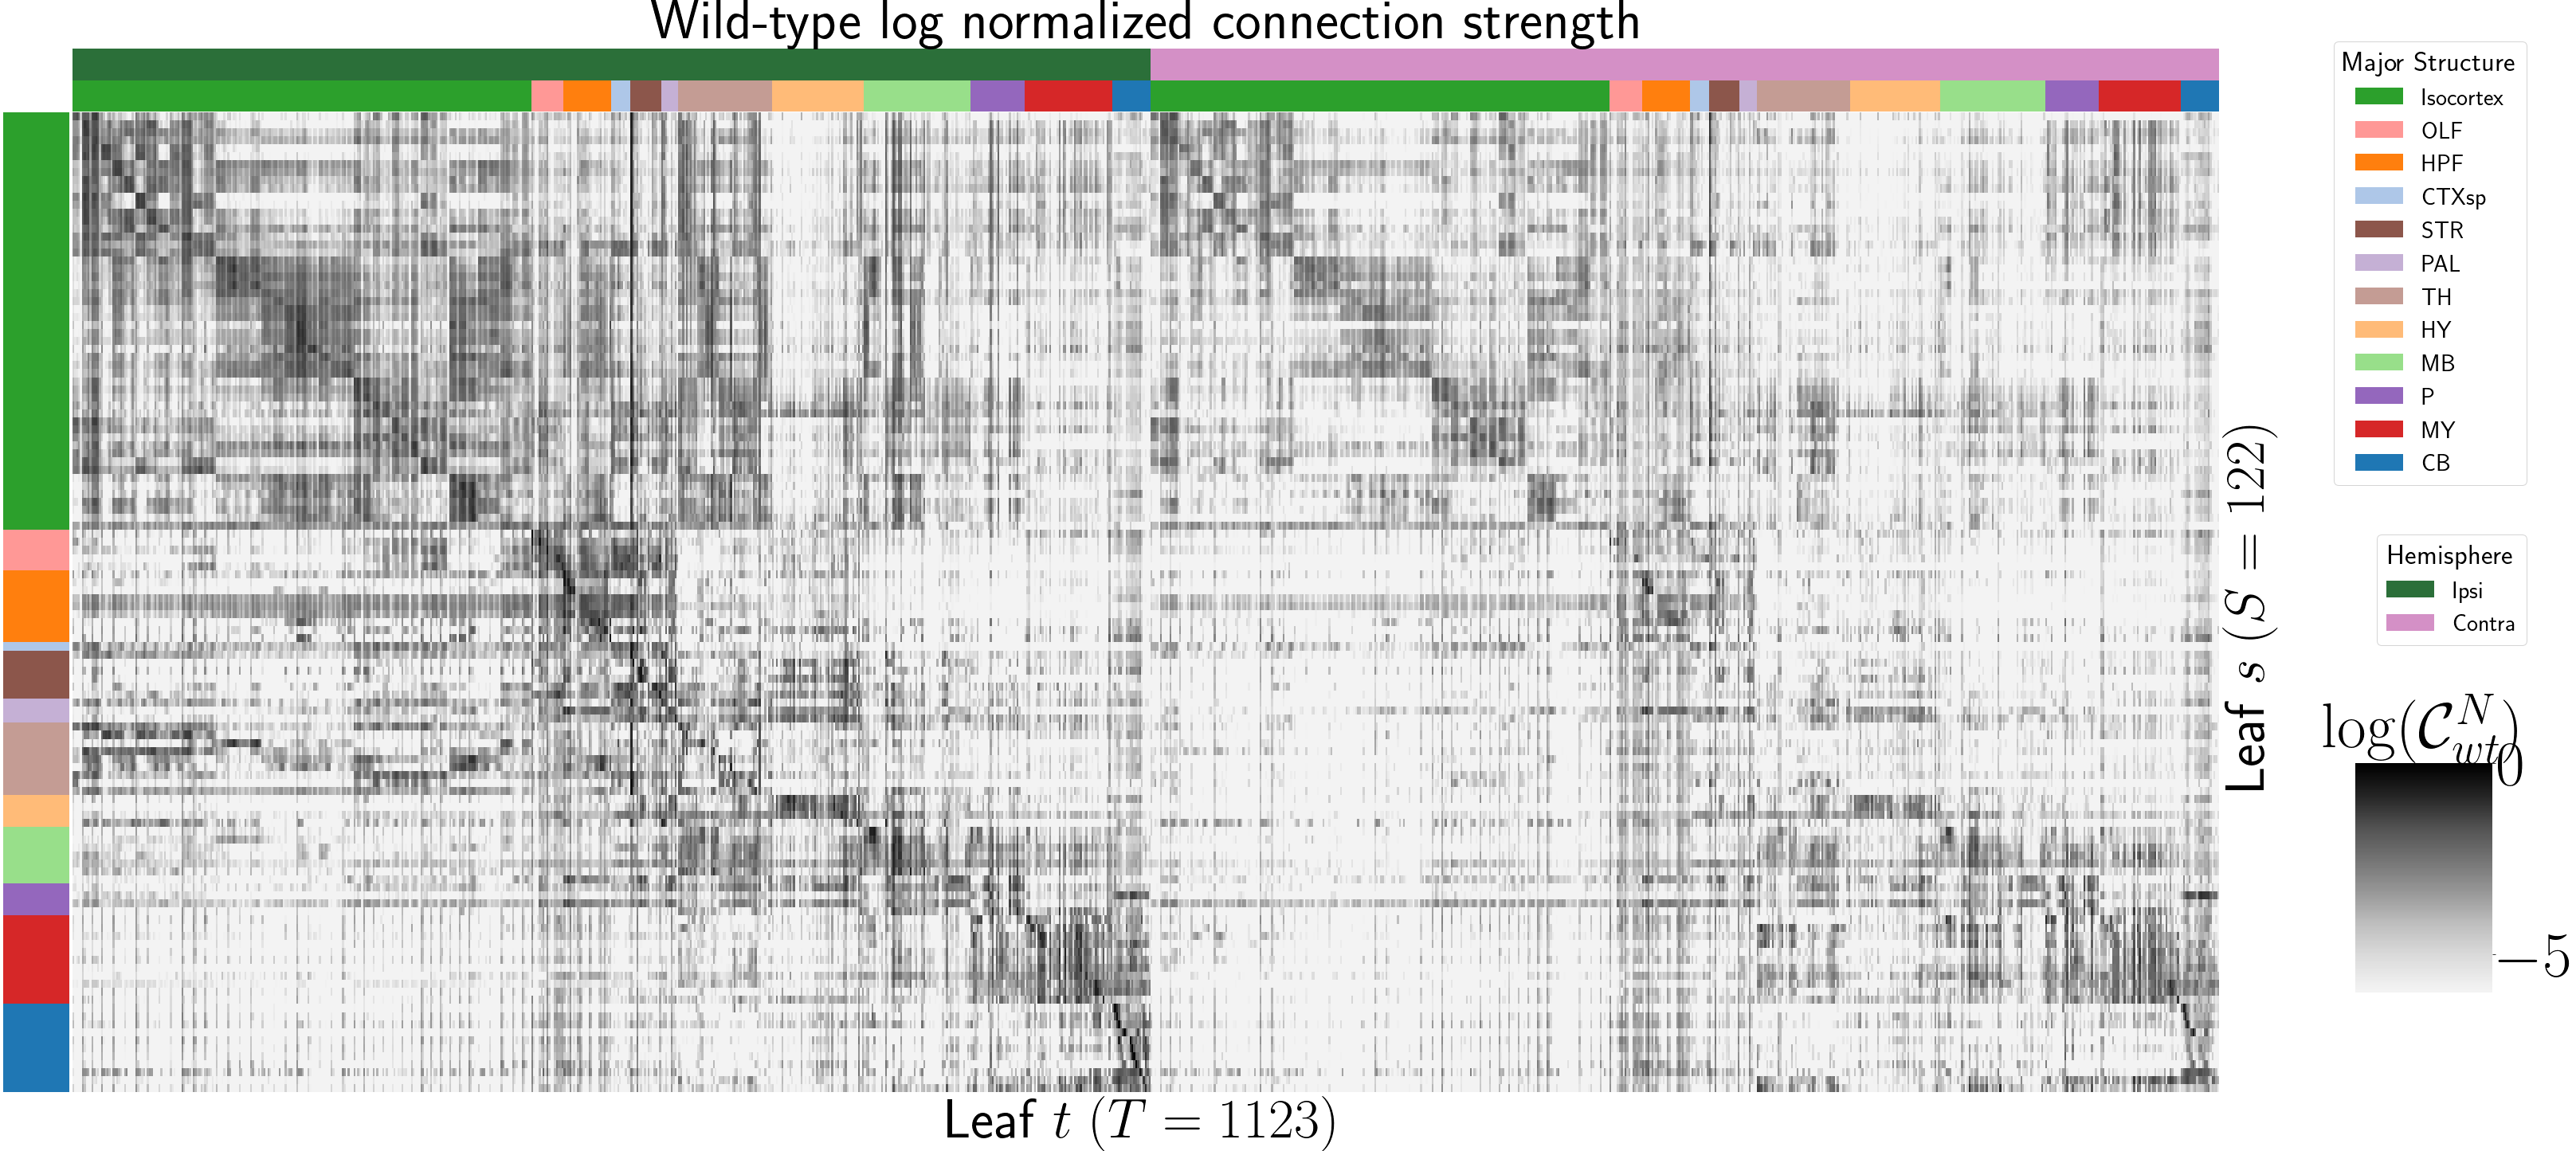
\includegraphics[width = \textwidth]{figs/conn_leaf2.png}
    } 
        \newline
       \subfloat[] {
    \label{fig:cortex_wt}
    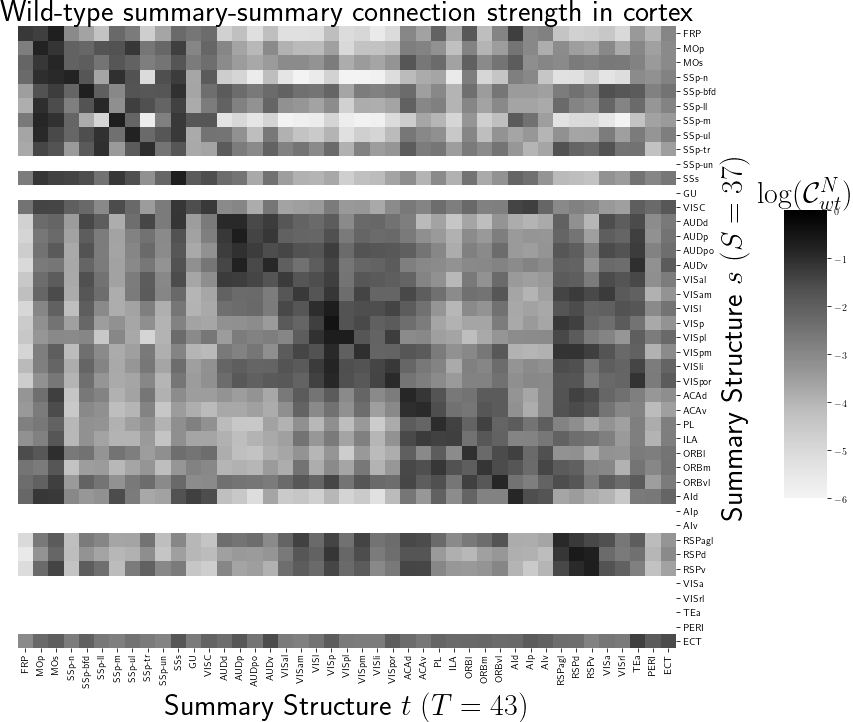
\includegraphics[width = .5\textwidth]{figs/conn_sum_cortex.png}
    } 
   \caption{Wild-type connectivities.
   \ref{fig:full_wt} Log wild-type connectivity matrix $\log \mathcal {C} (s,t,v_{wt})$.
   \ref{fig:cortex_wt} Log wild-type intracortical connectivity matrix at the summary structure level.}
   \label{fig:connectome}
\end{figure}

\newpage
\subsubsection{Class-specific connectivities}

Source and cell-type combinations which project similarly indicate the network structure underpinning cognition.
Our estimates of these class-specific connectivities exhibit certain known behaviors.
In Figure \ref{fig:data_ct}, we display results for the VISp and MO cortical areas.
These are ideal testbeds for our connectivities because they have well-established layer-specific projection patterns that can be detected with our layer-specific Cre-line based targeting \citet{Jeong2016-dc}, and are also well-represented in our dataset.

Our results are consistent with anterograde tracing experiments outside our dataset \citet{Jeong2016-dc}.
Figure \ref{fig:ct_spc} shows that in VISp, the Ntsr1-Cre line strongly targets the thalymic LP nuclei, and in MO, layer 5 projects to anterior basolateral amygdala (BLA) and capsular central amygdala (CEA), while layer 6 does not.
Recall that we display connectivity estimates for structures with at least one injection centroid in the structure.
Thus, the position of non-zero rows in Figure \ref{fig:ct_spc} shows the localization of Rbp4-Cre and Ntsr1-Cre injection centroids to layers 5 and 6 respectively (this is further examined in Supplemental Figure \ref{fig:iso_count}).
Thus, as a heuristic alternative model, to also synthesize information about leafs targeted by different Cre-lines, we also generate an average connectivity matrix over all Cre-lines.
This model is not evaluated in our testing, and is only a general stand-in for overall behavior, but provides a useful summary of results.

Cell-class, while often correlated with cortical layer, is often a stronger driver of connectivity than summary structure.
Figure \ref{fig:ct_clust} shows a collection of connectivity strengths generated using cre-specific models for wild-type, Cux2, Ntsr1, Rbp4, and Tlx3 cre-lines from visual signal processing leafs in the cortex to cortical and thalymic nucleii.
We use heirarchical clustering to sort source structure/cell-class combinations by the similarity of their structural projections, and sort target structures by the structures from which they receive projections.
Examining the former, we can see that the Ntsr1 Cre-line distinctly projects to thalymic nucleii, regardless of summary structure.
This contrasts with the tendency of other cell-classes to project intracortically in a manner determined by the source structure.
Similarly, layer 6 targets are not strongly projected to by any of the displayed Cre-lines.
There are too many targeted summary structures to plot here, but we expect that the source profile of each target clusters by structure.

\newpage

\begin{figure}[H]
\subfloat[]{
\label{fig:ct_spc}
    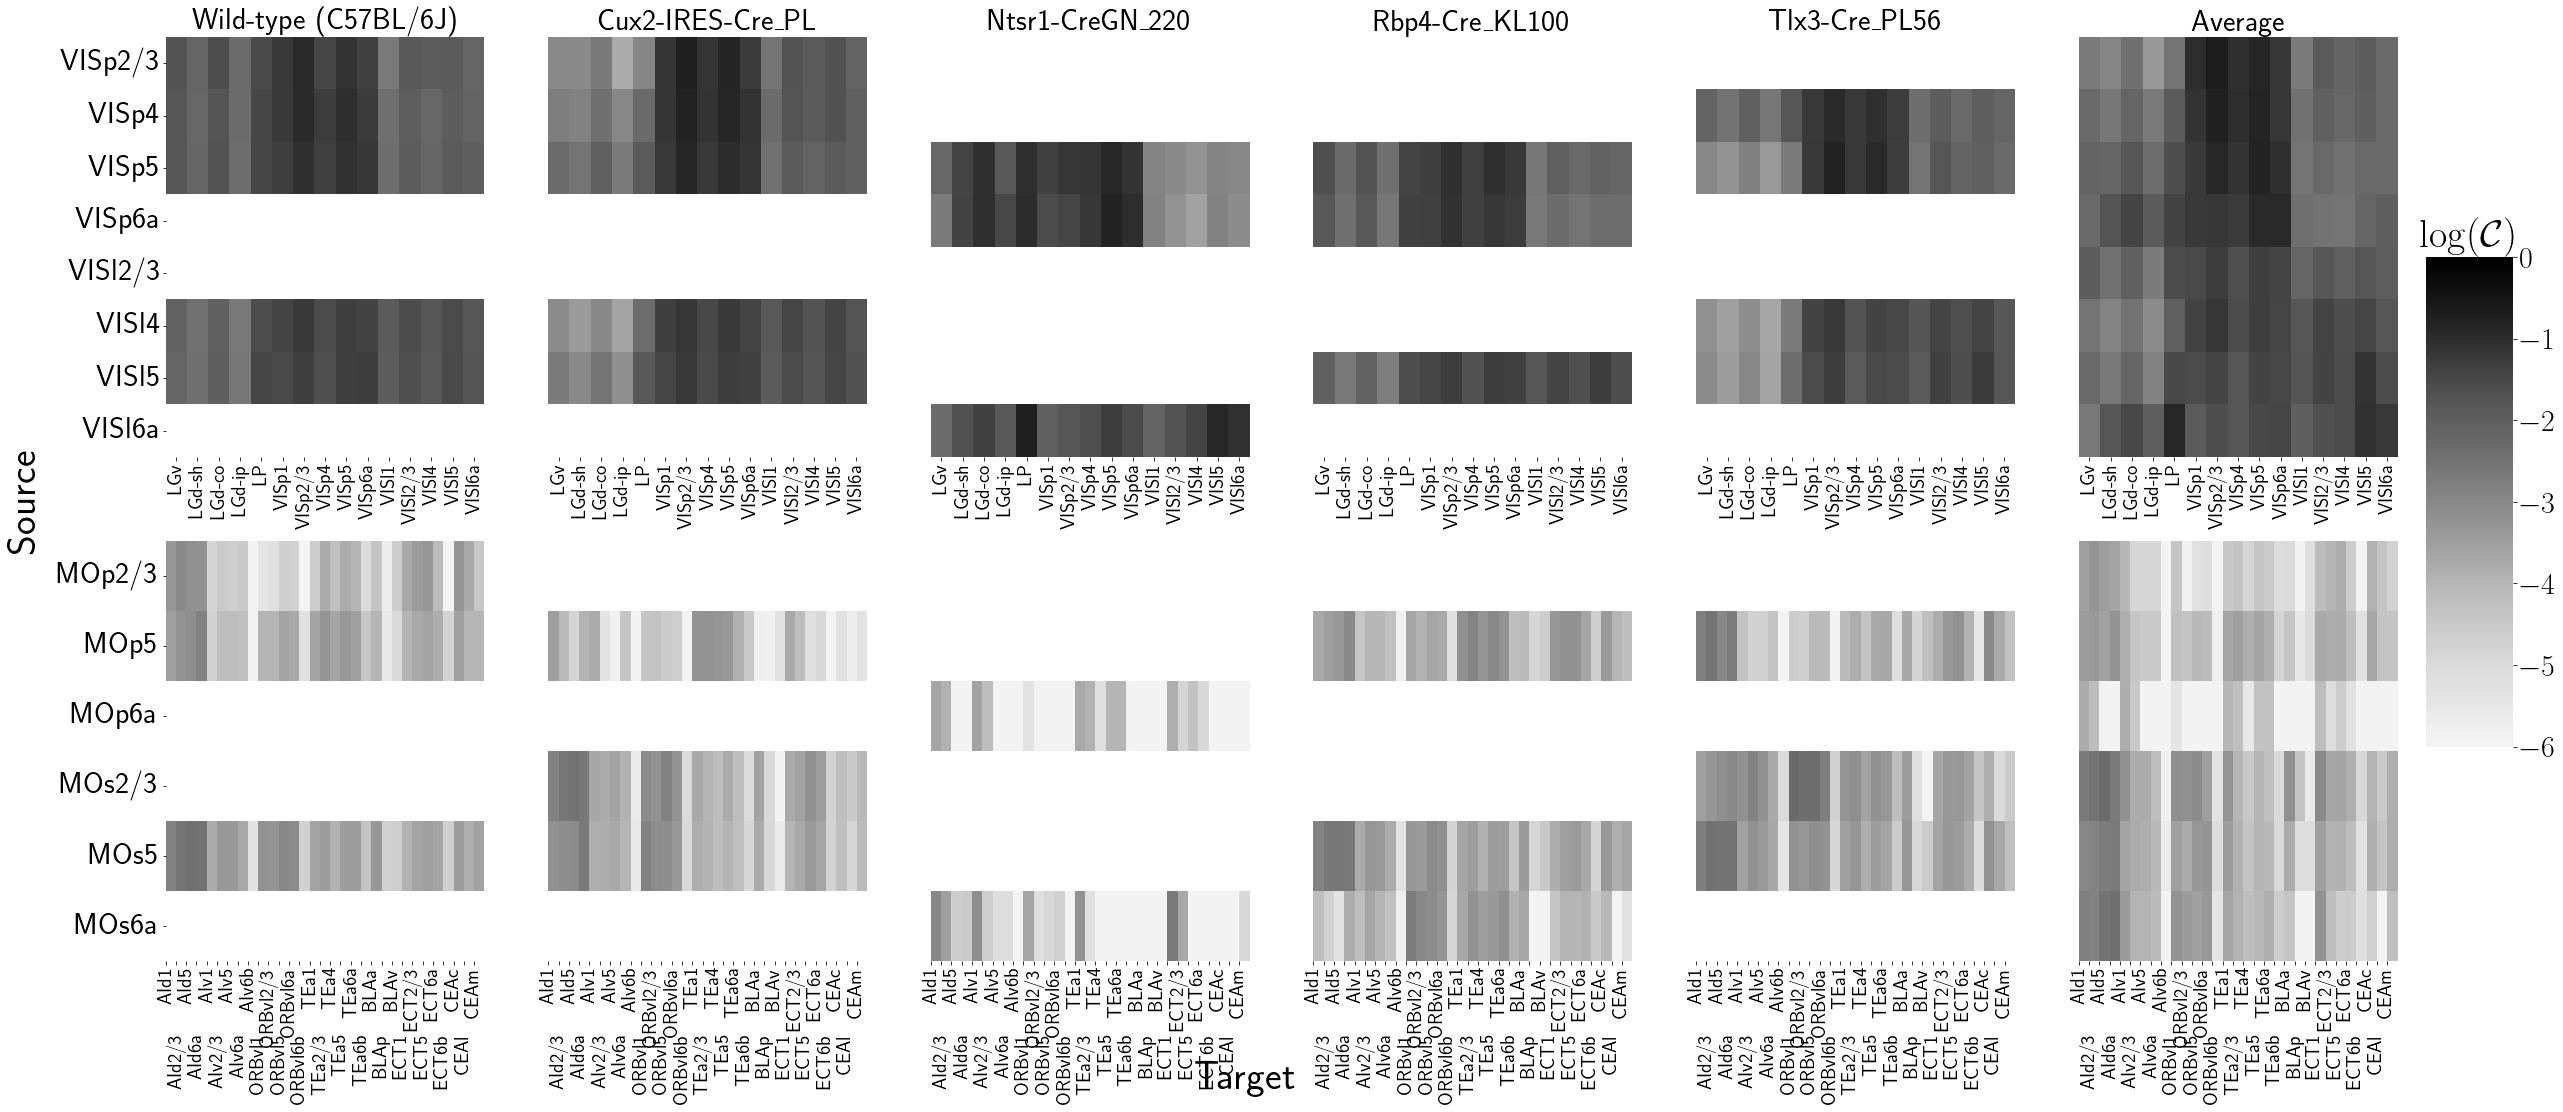
\includegraphics[width=.8\textwidth]{figs/visp_mo.png} 
    }
    \newline
 \subfloat[]{
 \label{fig:ct_clust}
    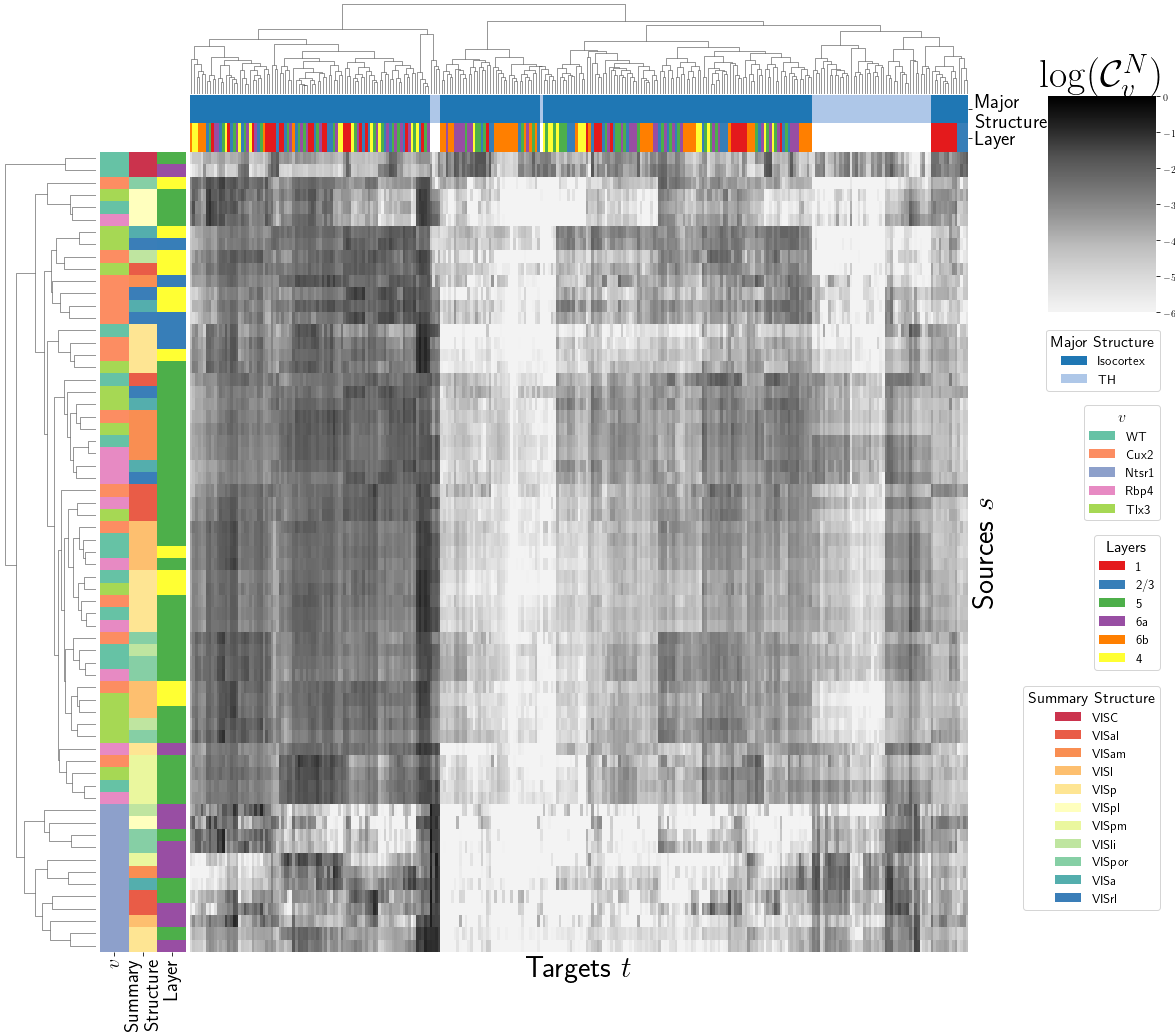
\includegraphics[width=.6\textwidth]{figs/heirarchical.png}
    }
    
    \caption{  Cell-class specificity. \ref{fig:ct_spc} Selected cell-class and layer specific connectivities from VISp and MO.
	 Sources without a injection of that Cre-type are not estimated due to lack of data for that Cre-line in that structure.
    		\ref{fig:ct_clust}
		Heirarchical clustering of connectivity strengths from visual signal processing cell-types to cortical and thalymic targets.
		Cre-line, summary structure, and layer are labelled on the sources.
		Major brain division and layer are labelled on the targets.}
\label{fig:data_ct}
\end{figure}

\newpage

\subsection{Connectivity Analyses}

Each structural connectivity matrix is a high-dimensional realization of relatively few biological processes, and decomposition of neural signals to recover these processes is a fundamental goal in neuroscience.
In this section, we apply non-negative matrix factorization to decompose the long-range wild-type connectivities into linear combinations of archetypal connectivities.
This decomposes the remaining censored connectivity matrix into a linear model based off a relatively small number of distinct signals.
This model is able to capture a large amount of the observed variability, and recovers structure-specific archetypal signals.

These signals are plotted in Figure \ref{fig:nmf_results}, and technical details and intermediate results are given in Supplemental Sections \ref{supp_sec:matrix_factor_methods} and \ref{supp_sec:matrix_factor_results}, respectively.
These details include a cross-validation based method for selecting the number of components, a masking method for focusing only on long range connections, and a stability method for ensuring that the decomposition is reliable across computational replicates.
The plotted decomposition shows that these underlying connectivity archetypes correspond strongly to major brain division.
However, certain components that predominantly represent connectivity from a given major brain division may also be accessed from other areas.
For example, the IP and FN regions of CB are strongly associated in \ref{fig:W} with the component projecting to MY in \ref{fig:H}.

Inspection of the reconstructed distal normalized connection strength using the top $15$ components shows qualitatively shows that this relatively sparse decomposition is able to capture much of the observed variability.
Layer-specific targeting is evident, indicating that the factorization method is detecting cell-type specific signals, even though it is trained only on the wild-type connectivity.
Other connectivity patterns like cortical-cortical and cortical-thalymic are also detected.

\newpage

\begin{figure}[H]
\centering
\hspace{1cm}
\subfloat[]{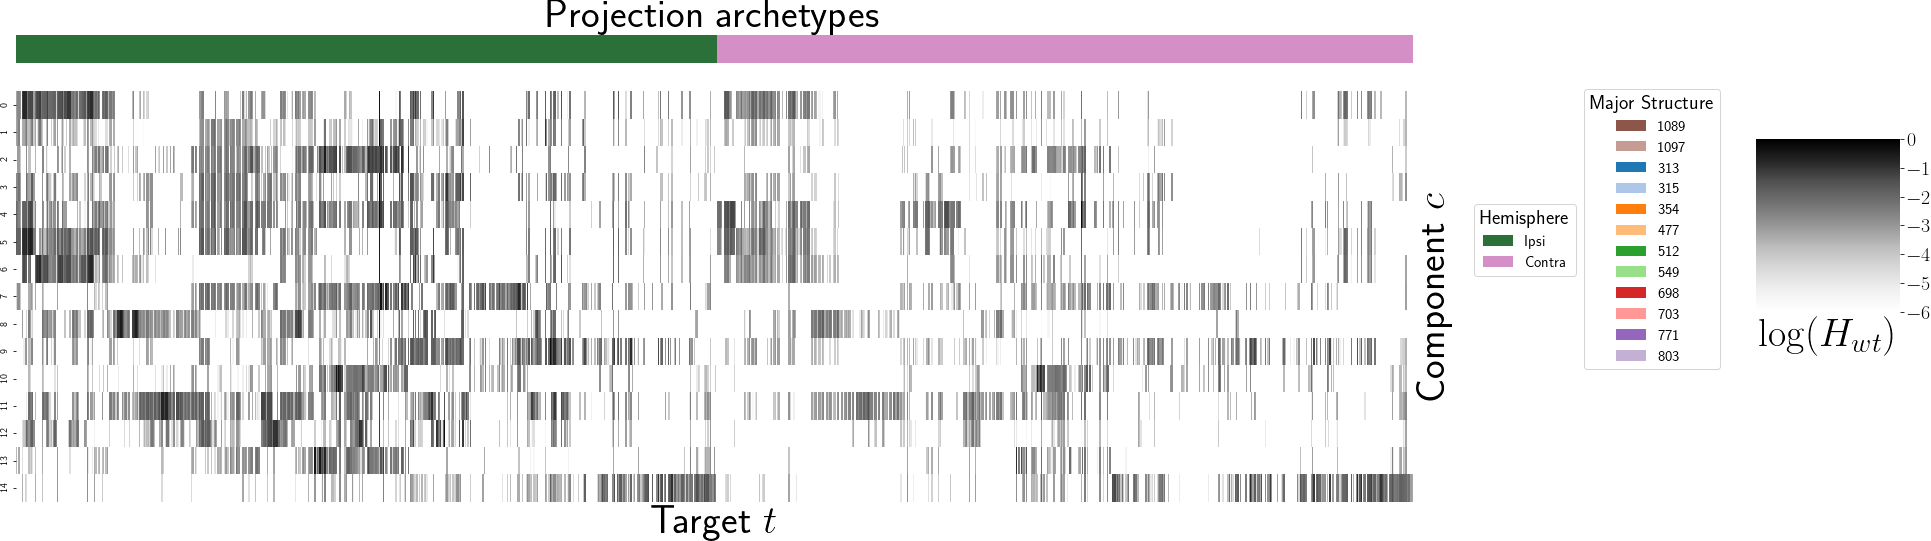
\includegraphics[width = .85 \textwidth]{figs/H_wt.png}
\label{fig:H}} 
\newline
\begin{tabular}[t]{cc}
\adjustbox{valign=t}{\subfloat[]{
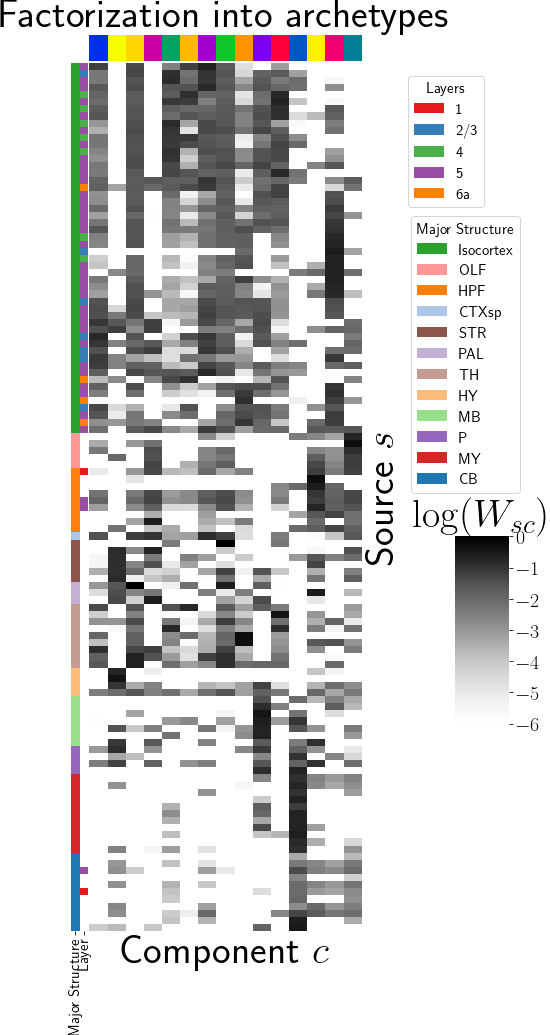
\includegraphics[width = .3\textwidth]{figs/W_wt.png}
\label{fig:W}}
} & 
\adjustbox{valign=t}{\subfloat[]{
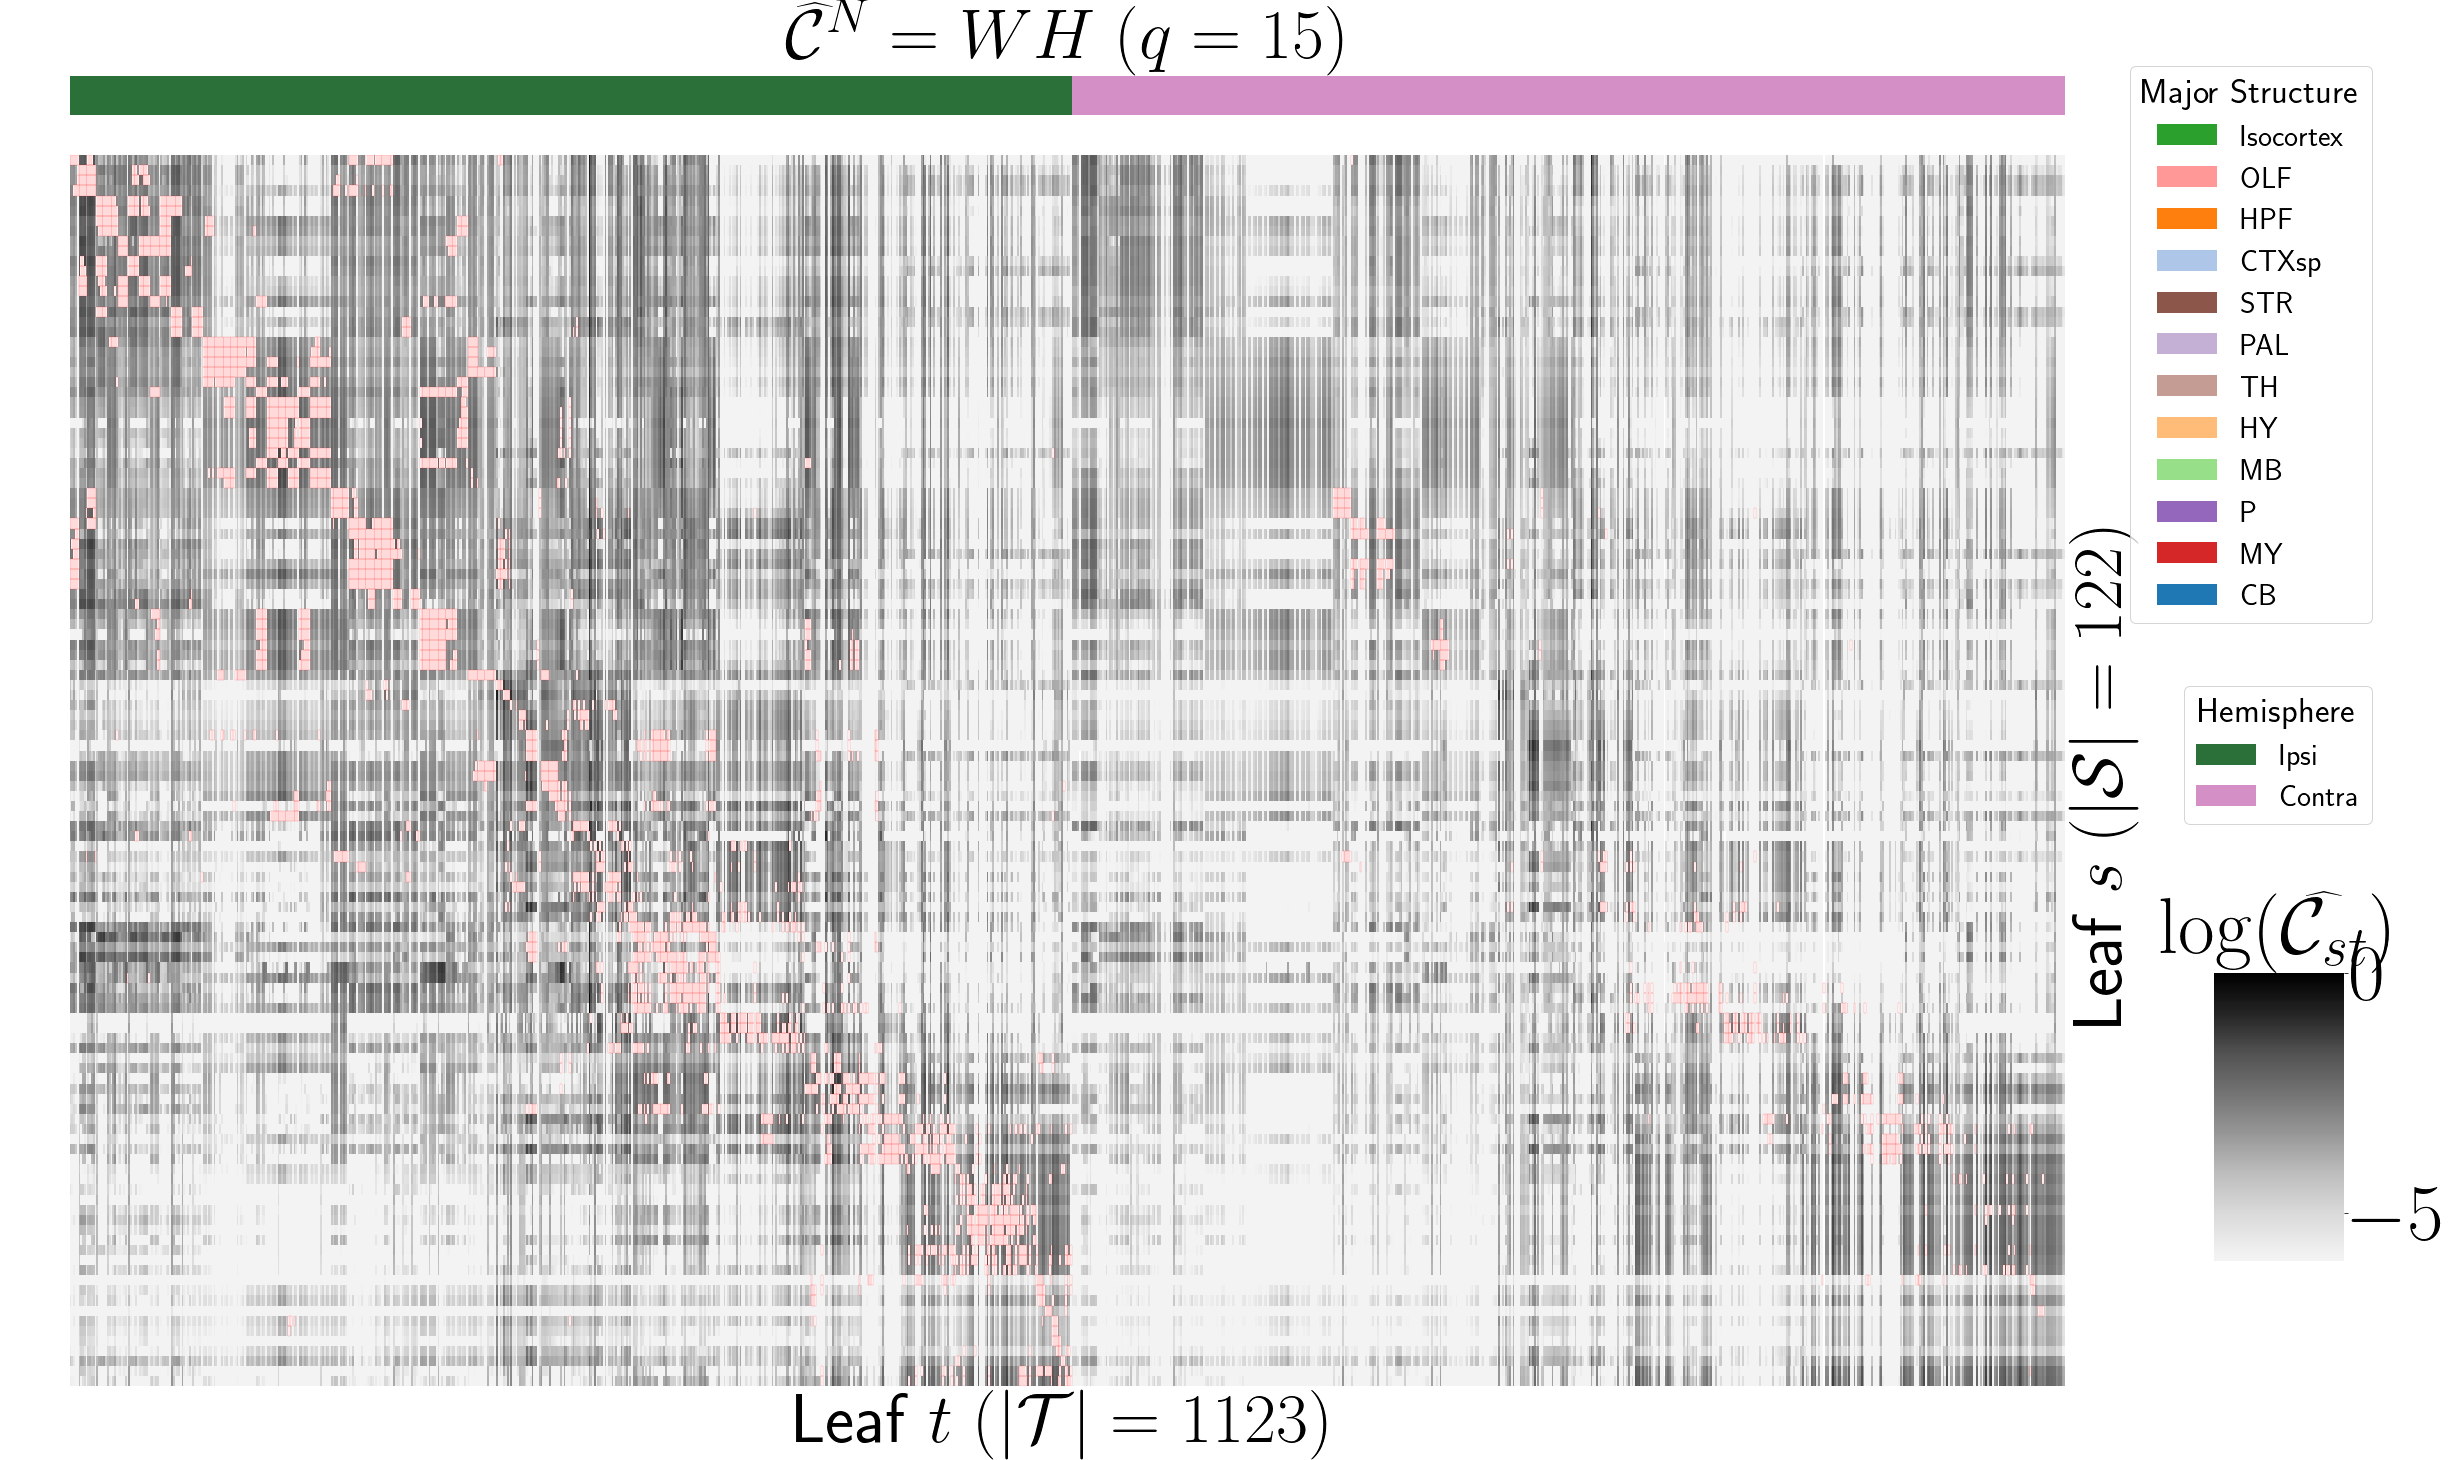
\includegraphics[width = .7\textwidth]{figs/conn_leafs_recon.png}
\label{fig:recon}}
} 
\end{tabular}
\caption{Non-negative matrix factorization results $\mathcal C_{wt}^N = WH$ for $q = 15$ components.
\ref{fig:H} Latent space coordinates $H$ of $\mathcal C$.
Target major structure and hemisphere are plotted.
\ref{fig:W} Loading matrix $W$.
Source major structure and layer are plotted.
\ref{fig:recon} Reconstruction of the normalized distal connectivity strength using the top $15$ archetypes.  Areas less than $1500 \mu m$ apart are not modeled, and therefore shown in red.
}
\label{fig:nmf_results}
\end{figure}

\newpage


\section{Discussion}

We see several opportunities for improving on our model.
Our particular task of transforming the injection and projection signal depending on cell-type is a non-linear transformation problem with categorical covariate.
Model averaging based off of cross-validation has been implemented in \citet{Gao2016-qe}, but we note that our approach makes use of a non-parametric estimator, rather than an optimization method for selecting the weights \citep{Saul2003-th}, and is applied specifically to a target-encoded feature space.
The properties of this estimator, as well as its relation to estimators fit using an optimization algorithm, are a possible future avenue of research.
Therefore, a deep model such as \citet{Lotfollahi2019-tr} could be appropriate, provided enough data was available.
With respect to the model, a Wasserstein-based measure of injection similarity per structure would combine both the physical simplicity of the centroid model while also incorporating structural knowledge.
Residual models of the above could also be considered.

The factorization of the connectivity matrix could be similarly improved.
Flattening $\mathcal C$ prior to unsupervised analysis is not necessarily recommended, but provides an easy solution for this problem.


%The Nadaraya-Watson weighting procedure introduced here is, to our knowledge, novel. 

%We make a key assumption: that the additional statistical accuracy of including more samples makes up for the fact that their expected accuracy is lower.
%Note that this assumption can be easily violated, if, for example, the data is distributed on a circle without error, and only nearest neighbors are most predictive.


%\skcomment{CITE METHOD THAT SELECTS WEIGHTS IN KERNEL (has catchy name)}


%The major-structure specific Nadaraya-Watson estimator from $\citet{Knox2019-ot}$ nevertheless appears poorly adapted for our circumstances since it does not take into account the virus $v$. It is not straightforward to include the viral strain in either $f_{NW}$ or $f_{NNLS}$. For $f_{NW}$, it is not clear how a one-hot encoded class-membership feature should be weighted. For $f_{NNLS}$, our sample size seems too low to utilize a fixed or mixed effect, particularly since the impact of the virus depend on the particular injection region, motivating use of an interaction term.


%%%%%%%%%%%%%%%%%%%%%%%%%%%%%%%%%%%%%%%%%%%%%%%%%%%%%%%%%%%%%%%%%
%%% End of Article

% \acknowledgments
% \section{Supporting Information} (optional)
% \section{Competing Interests} (optional)
% \bibliography{<name of .bib file>}





\acknowledgments
The Funder and award ID information you input at submission will be introduced by the publisher under a Funding Information head during production. 
Please use this space for any additional acknowledgements and verbiage required by your funders.

\section{Supporting Information}
This is an optional section. Please use this space to provide information about any supporting information referred to in your manuscript.

\section{Competing Interests}
This is an optional section. If you declared a conflict of interest when you submitted your manuscript, please  use this space to provide details about this conflict.


\bibliography{bibsamp}

\section{Technical Terms}

All NETN article types require Technical Terms.

Identify approximately 10 key terms that are mentioned in your article and whose usage and definition may not be familiar across the broad readership of the journal. 
Provide brief (20-word or less) definitions for each term, avoiding in these definitions the use of jargon, or highly technical or specialized language. 
When the article is typeset, the Technical Terms will appear in the margins at or near their first mention in the text.

In your manuscript, bold the first occurrence of each \textbf{Technical Term} and then provide a list of the terms and their definitions at the end of the manuscript after the references. 

\textbf{Technical Term} a key term that is mentioned in an NETN article and whose usage and definition may not be familiar across the broad readership of the journal. 

\end{document}


%\begin{algorithm}[h]{\label{alg:2stage}}
%\caption{2-stage estimator (Injection centroids $c(1:n)$, normalized projections $n(r(y(1:n)))$, viruses $v(1:n)$, target centroid $c$, target virus $v$)}
%\begin{algorithmic}

%\State Get structures $s(1:n) = r(c(1:n))$, $s = r(c)$
%\State Target encode $v(1:n)$ and $v$ with $n(r(y(1:n)))$
%\State Estimate expected loss $l_{ii'} = \hat f (\|c(i) - c(i')\|_2^2, \|t(v(i)) - t(v(i'))\|_2^2)$
%\State Return $\tilde y(i)$ (optional $\tilde x(i)$ )
%\end{algorithmic}
%\end{algorithm}

%\begin{algorithm}[h]{\label{alg:conn_mat}}
%\caption{Construct connectivity matrix (Cre-line $v$, Models $f_{1:N} (c,v)$, positions $c(R_n)$)}
%\begin{algorithmic}
%\State 2
%\end{algorithmic}
%\end{algorithm}
%\newpage
